\documentclass[preprint,11pt]{elsarticle}
\usepackage{amsmath,amssymb,booktabs,graphicx,longtable}
\usepackage[hidelinks]{hyperref}
\usepackage{url}
\usepackage{lmodern}
\setlength{\emergencystretch}{2em}
\newcommand{\PVDefaultPositiveCoverage}{84.96}
\newcommand{\PVDefaultOverallCoverage}{89.96}
\newcommand{\PVTunedPositiveCoverage}{86.32}
\newcommand{\PVTunedPositiveGain}{12.77}
\newcommand{\PVDefaultPositiveGain}{21.32}
\newcommand{\RollingRollingGain}{0.00}
\newcommand{\RollingCoverage}{88.59}
\newcommand{\RollingLocal}{6.37}
\newcommand{\SharedRollingGain}{-0.84}
\newcommand{\SharedCoverage}{88.78}
\newcommand{\SharedLocal}{6.21}
\newcommand{\IssuedRollingGain}{0.17}
\newcommand{\IssuedCoverage}{89.01}
\newcommand{\IssuedLocal}{6.22}
\newcommand{\COPRollingGain}{-2.90}
\newcommand{\COPCoverage}{90.11}
\newcommand{\COPLocal}{5.57}

\journal{Neurocomputing}
\newcommand{\IS}{\operatorname{IS}}
\newcommand{\ind}{\mathbf{1}}
\newcommand{\clip}{\operatorname{clip}}
\begin{document}
\begin{frontmatter}
\title{Predictive information and delayed adaptation in conformal calibration of frozen time-series foundation models}
\author[a]{Haoxuanzi Yin\textsuperscript{\href{https://orcid.org/0009-0001-1166-2216}{iD}}}
\ead{3250102684@zju.edu.cn}
\author[b]{Fan Zhang\textsuperscript{\href{https://orcid.org/0009-0004-3509-7495}{iD}}\corref{cor1}}
\ead{f.zhang@zju.edu.cn}
\cortext[cor1]{Corresponding author.}
\affiliation[a]{organization={Zhejiang University},city={Hangzhou},country={China}}
\affiliation[b]{organization={State Key Laboratory of Ocean Sensing and Ocean College, Zhejiang University},city={Zhoushan},postcode={316021},country={China}}
\begin{abstract}
Online conformal calibration combines predictive information with feedback adaptation,
but complete-pipeline comparisons can confound their contributions. Holding forecasts
and observation schedules fixed, we study native quantiles, delayed update states and
tuning for time-series foundation models. Native-band conformalized quantile regression
(CQR) improves interval score by 9.98\% over matched, validation-tuned residual calibration
across 124 model--series pairs, with transfer evidence from traffic and exchange rates.
On the latter panel, an 8.43\% long-horizon issued/shared-state CQR gain falls to 0.99\%
when the grid includes smaller rates. Wide-grid issued ACI adds only 0.17\% average
score improvement over rolling CQR; optimistic updating instead trades a higher score
for better aggregate and local coverage. Exact clipping accounting quantifies associated
finite-time coverage costs. Reliability remains unresolved even when efficiency improves:
after matched tuning, photovoltaic positive-output score improves by
\PVTunedPositiveGain\%, but coverage is only \PVTunedPositiveCoverage\% at a 90\% target.
The findings distinguish persistent predictive-information gains from tuning-sensitive
adaptation gains and motivate rolling controls and subgroup reliability checks.

\end{abstract}
\begin{keyword}
Time-series foundation models \sep Conformal calibration \sep Delayed feedback \sep
Probabilistic forecasting \sep Conditional reliability
\end{keyword}
\end{frontmatter}

\section{Introduction}
Pretrained time-series models can be deployed without fitting a new forecasting model
for every consumer, substation or generating plant. Models in the Chronos, TimesFM and
Moirai families also produce quantiles, making prediction intervals available alongside
point forecasts \citep{ansari2024chronos,das2024timesfm,ansari2025chronos2,liu2025moirai2}.
These intervals are potentially useful for monitoring and planning, but their nominal
levels need not match empirical coverage on a particular deployment stream. Miscalibration
can have either sign; recent TSFM calibration studies do not support a universal
undercoverage diagnosis \citep{adler2025calibration}.

Two decisions arise when recalibrating a frozen model. The first is the information
used to construct a nonconformity score: a point residual, a scaled residual or a violation
of native quantile endpoints. The second is the rule used to update its threshold as
outcomes arrive. CQR \citep{romano2019cqr} and online conformal methods
\citep{gibbs2021aci,zaffran2022acits,bhatnagar2023saocp,angelopoulos2023pid,gibbs2024dtaci}
provide established ingredients for both decisions. However, comparing complete pipelines
can obscure whether a gain comes from native uncertainty information, the update rule,
the evaluation split or different amounts of available feedback. A third issue is the
resolution at which reliability is measured: satisfactory overall coverage can coexist
with poor coverage on an operationally relevant subset.

We keep base forecasts fixed and cross score constructions with update rules under
identical feedback schedules. The main panel contains four pretrained models and 31
series; separate renewable, multi-horizon, traffic and exchange-rate panels test transfer.
The contribution is empirical attribution: identifying which apparent gains survive
changes to the comparison, and what they imply for selecting a calibration layer.

Two findings organize the study. First, native predictive information retains value
under matched tuning, whereas most of a large delayed-state CQR advantage is explained
by access to smaller learning rates. Direct comparison with rolling CQR reveals that
additional adaptation offers a score--coverage tradeoff rather than a uniform benefit.
This refines the usual recommendation to tune competing methods equally: the rate
range must also accommodate their distinct delayed dynamics. Second, photovoltaic
score gains occur on positive outputs as well as zeros, but positive-output coverage
remains deficient even after tuning. The deployment implication is to evaluate proper
score components and operationally meaningful subgroups together. Figure~\ref{fig:core}
shows the main controller comparison before the methodological details.

\begin{figure}[!htbp]\centering
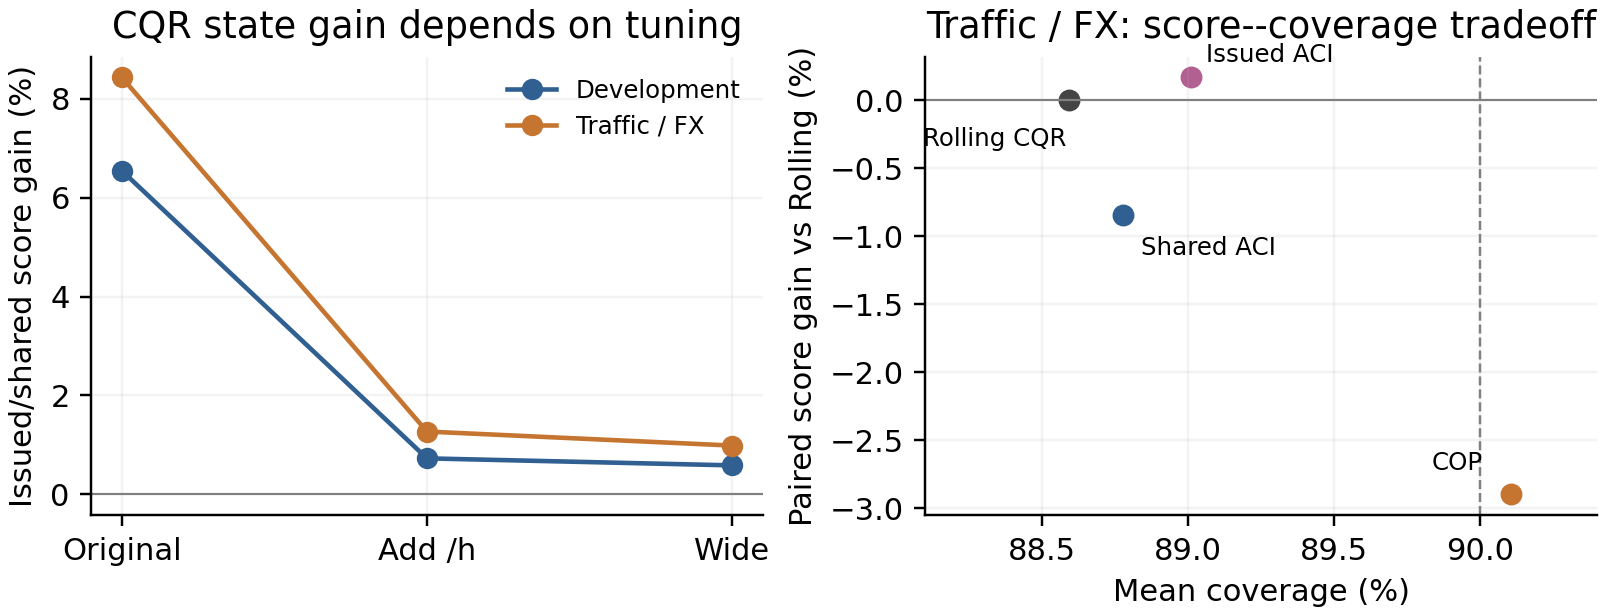
\includegraphics[width=\textwidth]{figures/core_findings.png}
\caption{Final controller findings at $h=24$. Left: paired issued/shared CQR gains
under three validation-selection grids. Right: direct paired gains over rolling CQR
versus mean coverage on traffic and exchange rates. All methods on the right use the
same native endpoints. ACI uses the wide grid; COP uses its declared delayed rate grid.
Points are panel summaries, not confidence regions or evidence of statistical equivalence.}
\label{fig:core}\end{figure}

The original family-confirmation experiment and subsequent sensitivities are kept
distinct in Table~\ref{tab:phases}. Established algorithms and classical stability
results provide the controls; no new calibration algorithm or validity theorem is
claimed. A source-checked multi-step PID configuration supplies an additional complete
method comparison, separate from the information-matched controller contrasts.

\section{Related work and scope}
CQR adapts interval endpoints using predicted quantiles \citep{romano2019cqr}, while
residual scaling is another established construction \citep{lei2018distfree}. Online
updates include ACI, adaptive aggregation, strongly adaptive experts, PID control and
decaying-step optimization \citep{gibbs2021aci,zaffran2022acits,gibbs2024dtaci,
bhatnagar2023saocp,angelopoulos2023pid,angelopoulos2024decay,areces2025online}.
Our common-forecast design compares these ingredients under explicit timing and
tuning choices. Declared adaptations and their implementation checks are given in
\ref{app:rules}; their original guarantees do not automatically transfer to modified,
clipped or delayed variants.

Foundation-model conformal prediction and native calibration are studied by
\citet{achour2025fm} and \citet{adler2025calibration}. Direct volatility modeling
\citep{cho2026volatility} and distribution-aware modularity \citep{schweizer2026dcp}
are close prior work. The present study adds controlled score--state--tuning contrasts
and output-regime diagnostics for fixed pretrained forecasts. Hidden-state-conditioned
calibration \citep{zhu2025afocp} requires representations absent from these archives.

Conformal Optimistic Prediction (COP) estimates the score distribution when updating
thresholds; its derivation already includes an implicit proximal objective
\citep{hu2026cop}. AcMCP models multi-step error autocorrelation and supplies multi-step
ACI and PID implementations \citep{wang2026acmcp}. Its ACI uses a shared state, whereas
the delayed recursion of \citet{elhalabi2026delayed} updates the issuing state.
Staggered integral control also studies delayed feedback \citep{cherenson2026staggered}.
We examine the practical consequences of these existing choices. O$^2$CP additionally
optimizes across horizons \citep{li2026o2cp}. Full AcMCP scorecasting and O$^2$CP are
not reproduced here; our configured multi-step PID comparison is consequently a
practical reference, not a comprehensive state-of-the-art ranking.

\section{A common causal calibration protocol}
\subsection{Information and time indexing}
At forecast origin $t$, the frozen model produces a point prediction $m_t$ and ordered
native quantiles for $Y_{t+h}$. Write $y_t=Y_{t+h}$ for the target associated with that
origin. Its outcome becomes observable to the calibrator after $h$ steps. More generally,
let $d\geq h$ be the feedback lag: at origin $t$, calibration may use only score/outcome
pairs with origins $i\leq t-d$. This convention includes the outcome revealed at the
current origin, but never the target being forecast.

Each trace has an excluded 600-pair calibration prefix followed by a 600-origin validation
prefix. All methods are evaluated from trace index 1200 onward, giving 2,999--14,199 test
origins in the main panel. At lag $d$, adaptive interval issuance begins at index $600+d-1$,
when all initial calibration outcomes are known. Validation losses use origins
$600+d-1,\ldots,1200-d$, so every label used for selection is available before testing.
Method states continue across the validation/test boundary. Static methods retain their
first-600 threshold; adaptive methods continue to learn. No method is evaluated on its
initialization outcomes.

The primary construction uses the stored 0.1 and 0.9 quantiles, denoted $\ell_t,u_t$,
even when the calibrated target is 90\%. A base band need not already have the final
nominal level to define a CQR score. In contrast, evaluating an \emph{uncalibrated native}
band requires matching its actual stored levels: a 0.1--0.9 band is nominally 80\%, not
90\%. No unrecorded tail quantiles are extrapolated. Quantiles are sorted within each
forecast to repair crossing; an unrearranged sensitivity uses the original stored columns.

\subsection{Scores and inversions}
Let $b_t=u_t-\ell_t$. We construct an outcome scale $v_t$ from a causal exponentially
weighted mean absolute error, updated only when a target is revealed, with decay 0.05.
Its initialization uses the first available forecast band and point prediction, not an
unseen outcome. The scale is bounded below by $10^{-12}$ for numerical arithmetic.
Define $\tilde b_t=\max(b_t,10^{-3}v_t)$. The four primary scores are
\begin{align}
 s_t^{\rm R}&=|y_t-m_t|,&
 s_t^{\rm E}&=|y_t-m_t|/v_t,\\
 s_t^{\rm N}&=|y_t-m_t|/\tilde b_t,&
 s_t^{\rm Q}&=\max(\ell_t-y_t,y_t-u_t).
\end{align}
They yield intervals $[m_t-q_t,m_t+q_t]$, $[m_t-v_tq_t,m_t+v_tq_t]$,
$[m_t-\tilde b_tq_t,m_t+\tilde b_tq_t]$ and $[\ell_t-q_t,u_t+q_t]$, respectively.
The native-scale control asks whether a native width helps without using native endpoints
directly; the past-error-scale control asks whether a simple outcome-based scale suffices.
CQR thresholds may be negative, allowing a band to shrink.

If inversion produces reversed endpoints, we record the event and emit a singleton at
their center. This is a practical interval repair rather than the exact empty set obtained
from signed-score inversion. Coverage-driven updates use the emitted interval. Infinite
intervals, if produced, are counted and retain infinite interval scores; they are not
capped or dropped. The primary CQR--ACI test intervals are singletons at an average rate
of 0.013\%, and no infinite intervals occur in the reported primary comparison.

We also examine normalized CQR, with denominator
$\max(b_t+\lambda v_t,10^{-3}v_t)$ for $\lambda\in\{0,0.01,0.1,0.5,1\}$.
A prefix selector chooses the lowest validation interval score among these five recipes
and the four primary scores under ACI. This is an existing model-selection principle used
as a diagnostic, not a proposed novel algorithm. A separate midpoint control replaces
$m_t$ by $(\ell_t+u_t)/2$ while retaining the residual or native-scale score.

\subsection{Update rules and implementation fidelity}
Rolling calibration inverts the empirical $(1-\alpha)$ quantile of the most recent
$W=450$ revealed scores. Clipped ACI instead uses $1-a_t$, with the default shared update
\begin{equation}\label{eq:aci}
a_t=\clip_{[0.001,0.999]}\{a_{t-1}+\gamma(\alpha-e_{t-d})\},\qquad\gamma=0.02,
\end{equation}
where $e_i=\ind\{y_i\notin C_i\}$ uses the emitted interval and updates start after
its feedback is revealed. The issuing-state alternative is defined below.
The main panel additionally evaluates fixed-prefix, SF-OGD, PI-log, SAOCP and FACI-R
variants. Exact rules, signed-score extensions and source-fidelity checks are retained
in \ref{app:rules}. Original ACI tuning selects
$(\gamma,W)\in\{0.005,0.02,0.05\}\times\{200,450,900\}$ using validation only;
later state sensitivities hold the window fixed while varying rates.

\section{Delayed adaptation and finite-time coverage}
\subsection{Clipping changes the coverage accounting}
The standard telescoping argument for an unconstrained ACI update does not survive
clipping unchanged. Index revealed errors by $k$ and define the projection correction
$r_k=a_{k+1}-a_k-\gamma(\alpha-e_k)$. Summing this definition gives the exact identity
\begin{equation}\label{eq:identity}
 \frac{1}{K}\sum_{k=1}^K e_k-\alpha
 =\frac{a_1-a_{K+1}}{\gamma K}+\frac{1}{\gamma K}\sum_{k=1}^K r_k.
\end{equation}
The first term vanishes for bounded levels, but the second need not. Repeated projection
at the lower boundary can accumulate a positive correction and therefore excess
miscoverage. A finite delay also leaves pending outcomes at the endpoint; their contribution
to an issued-versus-revealed average is at most the pending fraction. The more important
finite-sample effect can be the evolution of the controller: several intervals issued
before corrective feedback arrives can produce a run of errors and repeated clipping.
Equation~\eqref{eq:identity} is an elementary accounting identity, not a new validity theorem.
It motivates recording clipping and testing lag separately from horizon.

\subsection{State choice changes the delayed linear response}\label{sec:topology}
Let $e_i$ denote miscoverage of the interval issued at $i$, and take $d=h$.
After the initialization period, two established update structures are
\begin{align}
 a_t^{\rm S}&=\clip\{a_{t-1}^{\rm S}+\gamma(\alpha-e_{t-h}),0.001,0.999\},\label{eq:shared}\\
 a_t^{\rm I}&=\clip\{a_{t-h}^{\rm I}+\gamma(\alpha-e_{t-h}),0.001,0.999\}.\label{eq:issued}
\end{align}
Each error belongs to the corresponding controller's emitted interval. The first
structure is shared-state updating; the second is issued-state updating
\citep{wang2026acmcp,elhalabi2026delayed}. They coincide at $h=1$. At larger horizons,
the second has $h$ interleaved state subsequences, although our common rolling score
history still couples the observations used by those subsequences.

Consider a deterministic local approximation with stationary differentiable
miscoverage response $M(a)$, $M(a^*)=\alpha$, and $g=M'(a^*)>0$. Assume clipping
is inactive and replace binary feedback by this response. Writing $x_t=a_t-a^*$
gives, respectively,
\begin{equation}
 x_t=x_{t-1}-\gamma g x_{t-h},\qquad
 x_t=(1-\gamma g)x_{t-h}.
\end{equation}
The classical scalar delay-difference stability boundary \citep{deger2017stability}
and the second recurrence give
\begin{equation}\label{eq:stability}
 0<\gamma g<2\sin\!\left(\frac{\pi}{4h-2}\right)\quad\text{(shared)},
 \qquad 0<\gamma g<2\quad\text{(issued)}.
\end{equation}
For the shared recurrence, the characteristic polynomial is
$z^h-z^{h-1}+\gamma g$; its first unit-circle crossing has angle
$\pi/(2h-1)$. For the issued recurrence, calendar-time contraction is
$|1-\gamma g|^{1/h}$. Thus the wider gain range does not imply rapid tracking.
These familiar linear facts supply an explanatory approximation, not a new theorem
for stochastic empirical-quantile feedback, changing score windows, atoms or clipping.

Clipping accounting also depends on state choice. For the interpolation with raw update
$(1-\rho)a_{t-1}+\rho a_{t-h}+\gamma(\alpha-e_{t-h})$, define the projection correction
$r_t$ and $V_t=a_t+\rho\sum_{k=1}^{h-1}a_{t-k}$. Direct subtraction yields
\begin{equation}\label{eq:potential}
 V_t-V_{t-1}=\gamma(\alpha-e_{t-h})+r_t.
\end{equation}
Shared and issued states correspond to $\rho=0$ and $1$. Over $K$ updates,
average excess miscoverage equals
$[\sum_t r_t-(V_{\rm end}-V_{\rm before})]/(\gamma K)$.
Bounded levels control the endpoint term, but do not remove the accumulated clipping
correction. Neither state decomposition nor local stability proves coverage of the
practical clipped implementation.

\section{Experimental design}
\subsection{Series and frozen models}
The main panel comprises ten hourly UCI electricity consumers; eight Alabama photovoltaic
series sampled every ten minutes; four ETT channels, including three oil-temperature
channels and one load channel; and ERCOT total, COAST and NORTH hourly load. These are
25 observed energy-related series. We additionally include two cross-consumer splices,
two concatenations of seasonal windows and two synthetic regime-switching series, for
31 in total. Constructed switches and discontinuous seasonal concatenations are stress
tests, not naturally continuous deployment records. ETT minute-level data are sampled
every 15 minutes. We neither call every channel a load series nor describe all 31 series
as independent real energy datasets. Dataset identifiers and construction details are
provided in \ref{app:data}.

The archived model labels are Chronos-Bolt-base, Chronos-2, TimesFM-2.0-500M and
Moirai-2.0-R-small. Forecasting uses a 512-observation context, starts at raw-series index
600, and performs no task-specific parameter training. Within each series, all four
archives have the same targets and origin indices. An independent check against the
local raw loaders found a maximum absolute target-alignment error below $10^{-8}$ across
all 304 archive/horizon instances used by the four archive panels.

The evidence uses archived predictions. Exact local spot checks cover 84 model--origin
cases; full multi-horizon generation and confirmation provenance are retained.
Original checkpoint metadata remain incomplete, and pretraining exclusion cannot
be established. Details are in \ref{app:integrity}.

A separate GEFCom2014 panel \citep{hong2016gefcom2014} includes three solar and ten wind
zones with three available model archives, giving 39 pairs. It assesses transfer to
different renewable series, while retaining possible dependence among zones. The
multi-horizon panel contains eight series and two Chronos backbones at $h=1,6,24$, giving
48 model--series--horizon combinations. Its solar horizons correspond to 10 minutes,
one hour and four hours; 24 steps is day-ahead only for the hourly series. A dense-output
sensitivity uses 93 existing archives, without treating them as additional independent
datasets.

\subsection{Confirmation families and stronger controller controls}\label{sec:confirmationdesign}
The subsequent confirmation panel uses four traffic columns (0, 20, 40, 60) and four
exchange-rate columns (0, 2, 4, 6), with zero-based indices from the author benchmark
repository\footnote{\url{https://github.com/laiguokun/multivariate-time-series-data}}.
The source describes hourly road occupancy and daily exchange-rate observations.
We use the first 8,000 traffic observations and all 7,588 exchange-rate observations,
without outcome-dependent column selection or imputation. In the latter case, a
24-step horizon means 24 recorded observations, not necessarily 24 calendar days.
The two Chronos backbones yield 16 model--series pairs at each evaluated horizon.
These families were absent from calibration development; the public data may still
have appeared in neural pretraining. The protocol was fixed locally before their
download and test evaluation, not externally preregistered.

Forecasts are newly generated for every horizon from 1 through 24, using context 512,
batch size 128 and bfloat16 inference. We retain source commit and data hashes,
checkpoint/configuration hashes, target indices and runtime information. The same
generation procedure reproduces all stored point and quantile values at $h=1,6,24$
for the 16 original multi-horizon archives. The confirmation analysis evaluates
$h=1,6,24$ with the same initial calibration, validation and test-origin boundaries.
Test counts are 6,176 per traffic trace and 5,764 per exchange-rate trace.

For both residual and CQR scores, the confirmation panel compares rolling quantiles,
shared and issued ACI, PI-log, SF-OGD, COP, grouped ACI, fixed-scale quantile-gradient
updating, and an implicit-update ablation. ACI uses a 450-score window and selects
$\gamma\in\{0.005,0.02,0.05\}$ on validation interval score. PI-log and SF-OGD use
the declared fixed defaults rather than being described as tuned optima.
COP selects from $\{0.05,0.1,0.5,1\}$ and those rates divided by $h$; its preceding
score-history range sets the step scale. Observable-width grouping is a separate
control. Their exact delayed recursions, initialization and grouping rules are in
\ref{app:rules}; the matched implicit control is in \ref{app:implicit}.

\subsection{Additional tuning sensitivity and multi-step PID}\label{sec:v8design}
After inspecting the confirmation results and reviewing tuning adequacy, we fix an
additional sensitivity protocol. Its original grid is $G_0=\{0.005,0.02,0.05\}$;
the scaled grid is $G_0\cup G_0/h$. The wide grid adds
$\{0.0001,0.0002,0.0005,0.001,0.002,0.005,0.01,0.02,0.05,0.1\}$ to the scaled grid.
Both states receive every candidate, with all other settings unchanged. Each grid
selects its own validation minimizer. We first execute the development panel and then
revisit the traffic/exchange-rate panel without modifying the grid. These are subsequent
exploratory sensitivities on inspected data, not extensions of the original locked
confirmation claim. Together they contain 4,608 computed configurations; all are retained.

The accompanying multi-step PID uses signed errors and asymmetric tail intervals,
with four configured scorecasters and validation-selected rates, including $1/h$
scaling. Across both panels, 2,560 configurations are retained. Its accelerated
recursion matches the unmodified author code over all 24 horizons and four
scorecasters, and passes future-target perturbation checks. Exact settings are in
\ref{app:rules}. PID versus CQR changes both information and interval construction;
it is a complete-configuration comparison, not an isolated controller intervention.

\subsection{Metrics, aggregation and uncertainty}
The primary target is $1-\alpha=0.9$. For interval $[L_t,U_t]$, the standard interval
score is
\begin{equation}
 \IS_\alpha=(U_t-L_t)+\frac{2}{\alpha}(L_t-y_t)_+
                         +\frac{2}{\alpha}(y_t-U_t)_+.
\end{equation}
This proper score balances width and miss distance \citep{winkler1972,gneiting2007proper}.
At a fixed nominal level it remains meaningful when methods attain different empirical
coverage; coverage is reported alongside the score rather than used to dismiss a result.
We also report absolute coverage error per pair, lower and upper miss rates, mean width,
and the average absolute coverage error over rolling 150-origin windows. Overall coverage
and local error answer different questions, and neither establishes conditional coverage.

For each pair, relative gain is $100(1-\overline\IS_A/\overline\IS_B)$. We first average
gains across backbones for each series and then across series, avoiding the pooling of raw
scores measured in incompatible units. Unless otherwise stated, the denominator is that
pair's default residual--ACI score. Tuned-versus-tuned comparisons use the tuned residual
denominator explicitly. Confidence intervals on mean gains resample series 10,000 times;
they are descriptive for this panel, not geographic population intervals, because plants
and nested loads are correlated.

Within a pair, we use a paired moving-block bootstrap of per-origin score differences
with 1,000 resamples and block length 200, and check lengths 100 and 400. A centered
bootstrap test with a Monte Carlo correction is adjusted using Benjamini--Hochberg within
the 124 primary comparisons. Dependence across hypotheses can limit the nominal FDR
interpretation; adjusted counts are descriptive support, not 124 independent replications.
Family exclusions and per-family summaries are emphasized for generalization.

Confirmation summaries give equal weight to the two families, then their series and
backbones. We report paired relative gains, within-family medians and sign counts;
16 model--series pairs are not 16 independent datasets. No independent-dataset confidence
interval is attached to those counts. Each contrast names its own denominator.
For the photovoltaic diagnostic, zero versus positive target values are used only
after prediction to evaluate coverage. They do not route predictions, define validation
choices, or serve as a guaranteed conditional-coverage target. Observable-width groups
are distinct from these outcome-defined diagnostic groups.

\subsection{Analysis stages and comparison scope}
Table~\ref{tab:phases} separates development, the original confirmation and subsequent
exploration. Local protocols record decisions but are not external preregistration.
Information-matched state and rolling contrasts hold the endpoints, window and
reveal schedule fixed. Native-versus-residual contrasts hold the controller fixed.
Multi-step PID versus CQR instead compares complete configurations.

\begin{table}[!htbp]\centering\small
\caption{Analysis stages. Public data may have appeared in neural pretraining.}
\label{tab:phases}
\begin{tabular}{p{.19\textwidth}p{.33\textwidth}p{.38\textwidth}}\toprule
Stage & Data and role & Status of choices \\\midrule
Development & Historical main, renewable and multi-horizon archives & Retrospective;
fixed-forecast lag and midpoint checks added after inspection. \\
Original confirmation & Previously unused traffic and exchange-rate families &
Methods and grids fixed before download and test evaluation. \\
Subsequent sensitivity & Same development and confirmation panels & Wider rates,
configured PID, PV decomposition and rolling synthesis on already inspected data. \\\bottomrule
\end{tabular}\end{table}

\section{Results}
\subsection{What adaptation adds beyond rolling CQR}\label{sec:rolling}
Table~\ref{tab:rolling} compares each controller directly with rolling CQR on the
same 16 traffic/exchange-rate pairs at $h=24$. Wide-grid issued ACI gains only
\IssuedRollingGain\% on average; its median gain is approximately zero and only
6/16 pairs improve. The family means differ: traffic gains 1.26\%, whereas exchange
rates lose 0.92\%. Shared ACI loses 0.84\% on average. These paired calculations
avoid inferring gains by dividing separately averaged normalized scores.

\begin{table}[!htbp]\centering\scriptsize
\caption{Direct comparisons with rolling CQR at $h=24$, traffic/exchange rates.
Gain is the mean of $100(1-\IS_A/\IS_{\rm rolling})$ within each matched pair; positive
is better. Coverage is percent; Local is absolute 150-origin coverage error in
percentage points. Deltas subtract rolling values. ACI uses the wide grid.
Wins are descriptive signs, not independent significant replications.}
\label{tab:rolling}\begin{tabular}{lrrrrrr}
\toprule
CQR controller & Gain & Wins & Coverage & Local & $\Delta$ cov. & $\Delta$ local \\
\midrule
Rolling CQR & +0.00 & -- & 88.59 & 6.37 & +0.00 & +0.00 \\
Shared ACI & -0.84 & 2/16 & 88.78 & 6.21 & +0.18 & -0.16 \\
Issued ACI & +0.17 & 6/16 & 89.01 & 6.22 & +0.42 & -0.15 \\
COP & -2.90 & 6/16 & 90.11 & 5.57 & +1.51 & -0.80 \\
\bottomrule
\end{tabular}

\end{table}

Adaptation changes coverage as well as score. Issued ACI raises coverage from
\RollingCoverage\% to \IssuedCoverage\%, still below the 90\% target. COP has a
2.90\% higher score than rolling CQR, but reaches \COPCoverage\% coverage and reduces
local error from \RollingLocal\ to \COPLocal\ percentage points. This is a tradeoff,
not a single winner or an equivalence result. At zero learning rate, ACI initialized
at $\alpha$ keeps its level fixed and reduces to rolling score calibration with the
same window and timing. Frequent minimum-rate choices therefore have a useful
reference point: rolling continues to adapt its score distribution even without
level feedback. The small-rate results do not establish that a zero rate is optimal.

\subsection{Native bands help at one step, with a smaller benefit after fair tuning}
Table~\ref{tab:main} shows the primary comparison. CQR--ACI improves the interval score
by 13.57\% relative to residual--ACI, with a descriptive series-bootstrap 95\% interval
$[9.08,18.45]\%$. The gain is positive on 114 of 124 model--series pairs. Its mean
coverage is 89.98\%, and individual-pair coverage ranges from 89.82\% to 90.18\%.
The average absolute per-pair coverage error is 0.052 percentage points. Thus a near-target
grand mean is not merely cancellation of large positive and negative pairwise errors in
this particular comparison.

\begin{table}[htbp]\centering\small
\caption{Main panel at a 90\% target. Gain is relative to default residual--ACI.
Gap is the mean absolute pairwise coverage error; Local is the mean 150-origin coverage
error. FACI, SAOCP, SF-OGD and PI-log refer to the declared adaptations.}
\label{tab:main}\begin{tabular}{lrrrr}
\toprule
Score / rule & Gain (\%) & Cov. (\%) & Gap (pp) & Local (pp) \\
\midrule
residual/aci & 0.00 & 89.94 & 0.07 & 1.66 \\
error-scale/aci & 2.17 & 90.00 & 0.03 & 1.06 \\
native-scale/aci & 11.50 & 89.98 & 0.05 & 1.42 \\
cqr/aci & 13.57 & 89.98 & 0.05 & 1.45 \\
residual/faci & 8.57 & 89.19 & 0.81 & 1.86 \\
cqr/faci & 14.87 & 89.49 & 0.52 & 1.71 \\
residual/saocp & 3.32 & 92.54 & 2.64 & 2.92 \\
cqr/saocp & 12.40 & 90.73 & 1.49 & 2.07 \\
cqr/pi-log & 13.88 & 90.00 & 0.06 & 1.51 \\
cqr/sfogd & 13.28 & 90.00 & 0.03 & 0.98 \\
prefix-selected/aci & 13.72 & 89.98 & 0.05 & 1.46 \\
residual/aci/tuned & 5.23 & 89.74 & 0.28 & 1.65 \\
cqr/aci/tuned & 14.18 & 89.92 & 0.15 & 1.74 \\
\bottomrule
\end{tabular}
\end{table}

Native-scale ACI achieves an 11.50\% gain, whereas past-error scaling achieves 2.17\%.
This supports the value of native uncertainty beyond a simple causal residual-scale
estimate. It does not identify all of the CQR advantage with distributional shape:
the compared intervals differ in centering and additive versus multiplicative construction.
The exploratory midpoint-only residual control changes the gain to $-0.18\%$; using
native scaling around that midpoint yields 12.07\%. These controls indicate that
recentring alone does not explain the primary benefit. They do not establish a universal
decomposition of predictive uncertainty.

Validation tuning strengthens residual--ACI substantially: its gain against the default
is 5.23\%, while tuned CQR--ACI gains 14.18\% against the same default. Directly comparing
the two tuned methods gives a 9.98\% mean paired improvement. This is the relevant number
when asking whether CQR still helps after both methods select their ACI settings. It
would be misleading to quote 14.18\% as a gain against the tuned residual baseline.

Across the seven default rules, adding native information generally improves efficiency,
but the effects are not orders of magnitude apart (Figure~\ref{fig:rules}). FACI-R with
residuals already gains 8.57\% and has lower coverage, while residual SAOCP overcovers
on average. CQR--PI-log, CQR--SF-OGD and CQR--ACI have similar average interval scores
but different local errors. SF-OGD has the smallest mean local error among these three
one-step CQR variants. A universal assertion that the score renders the rule irrelevant
is therefore unsupported even before adding delayed feedback.

\begin{figure}[htbp]\centering
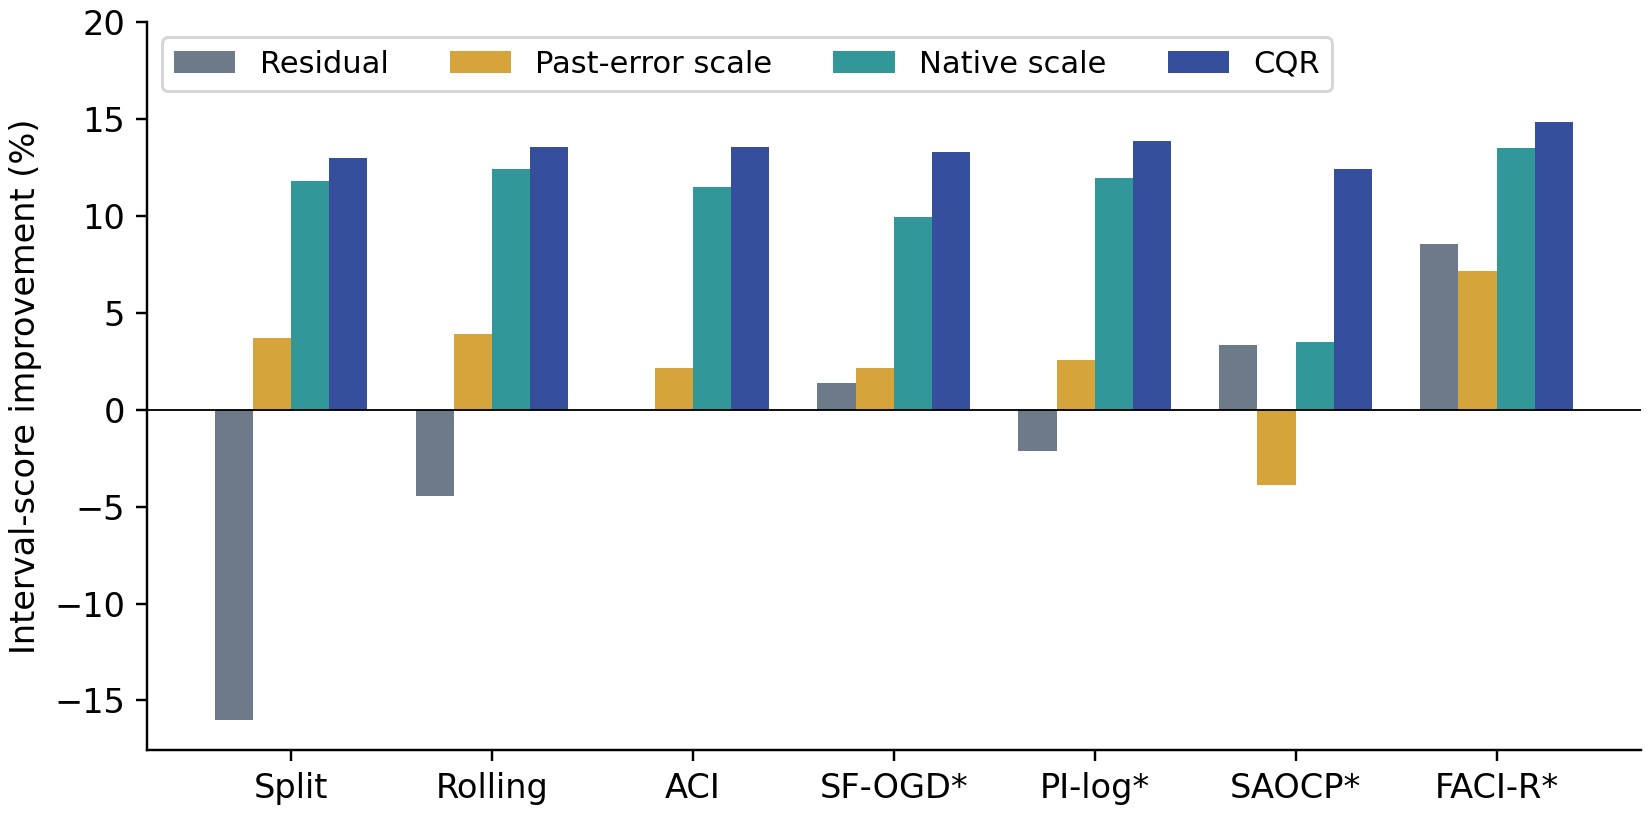
\includegraphics[width=\textwidth]{figures/score_rule.png}
\caption{Score--rule comparison on fixed one-step forecasts. Every gain uses the same
default residual--ACI denominator. Asterisks indicate the explicit adaptations described
in \ref{app:rules}; these labels do not claim equivalence to full original forecasting pipelines.}
\label{fig:rules}\end{figure}

\subsection{Benefits vary by family and persist on separate renewable series}
The mean CQR--ACI gain is 35.25\% on Alabama PV, 7.21\% on UCI loads, 5.96\% on ETT
and only 0.37\% on the three ERCOT loads (Table~\ref{tab:family}). The synthetic mean
is slightly negative. This heterogeneity is more informative than a pooled correlation
between a post-hoc volatility index and gains. Removing all eight PV series leaves
a 6.03\% gain, with descriptive interval $[4.25,7.88]\%$. Restricting to the 25 observed
series yields 15.16\%; that subset gives PV a larger relative weight. Leave-one-family-out
means remain positive, ranging from 6.03\% to 16.60\%.

\begin{table}[htbp]\centering\small
\caption{CQR--ACI gains by main-panel family. Intervals resample series within the listed
family and are descriptive; narrow intervals for correlated PV plants do not imply broad
geographic certainty. Small two- or three-series groups have especially limited precision.}
\label{tab:family}\begin{tabular}{lrrr}
\toprule
Family & Series & Gain (\%) & Descriptive 95\% CI \\
\midrule
Alabama PV & 8 & 35.25 & [34.75, 35.74] \\
Constructed seasons & 2 & 8.58 & [6.25, 10.90] \\
Constructed switches & 2 & 12.31 & [11.36, 13.27] \\
ERCOT & 3 & 0.37 & [-1.53, 1.86] \\
ETT & 4 & 5.96 & [3.41, 8.51] \\
Synthetic & 2 & -0.05 & [-0.42, 0.31] \\
UCI load & 10 & 7.21 & [5.53, 9.70] \\
\bottomrule
\end{tabular}
\end{table}
\begin{figure}[htbp]\centering
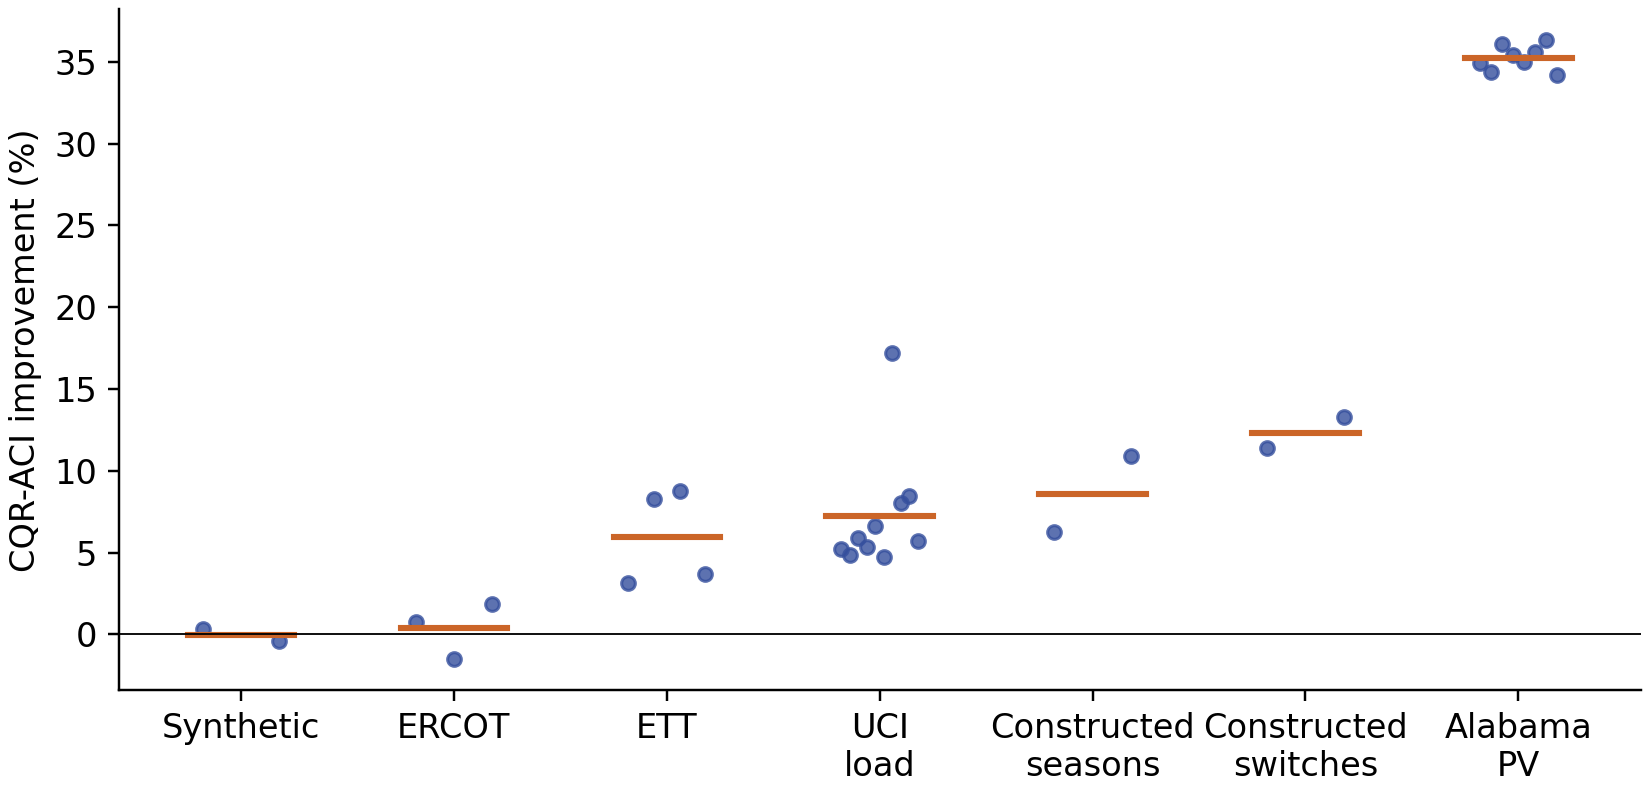
\includegraphics[width=\textwidth]{figures/families.png}
\caption{Each point is one series averaged across four backbones; horizontal orange marks
are family means. Constructed and synthetic series remain visible rather than being
counted as independent observed energy systems.}\label{fig:families}\end{figure}

Per-backbone mean gains are 15.15\% for Chronos-2, 13.82\% for Chronos-Bolt, 12.90\%
for Moirai and 12.41\% for the archived TimesFM configuration. On the separate GEFCom
panel, CQR--ACI gains 19.63\% overall: 41.46\% for solar and 13.08\% for wind, with
89.99\% mean coverage. This is evidence beyond the Alabama solar panel, but does not
convert correlated zones into independent geographic samples.

At block lengths 100, 200 and 400, 109 primary pairs have a positive paired-bootstrap
95\% interval and two have a negative interval. The centered-test/BH procedure identifies
109 positive and two negative differences at each of these block lengths. These counts
are reported with the dependence caveat above; the magnitude and family distribution of
the effect remain the main empirical evidence.

\subsection{Delayed feedback makes rule choice consequential}
Figure~\ref{fig:horizon} and Table~\ref{tab:horizon} show the joint horizon/feedback
experiment. At $h=24$, CQR--ACI has 87.34\% mean coverage, compared with 87.10\% for
residual--ACI. CQR--PI-log attains 89.96\% coverage and a 17.09\% score improvement
relative to residual--ACI, compared with 13.15\% for CQR--ACI. CQR--ACI's average number
of clipped updates, counting validation and test adaptation, increases from 3.06 at
$h=1$ to 201 at $h=24$. This is consistent with the projection term in
Equation~\eqref{eq:identity}, although a count alone does not measure its signed magnitude.

\begin{figure}[htbp]\centering
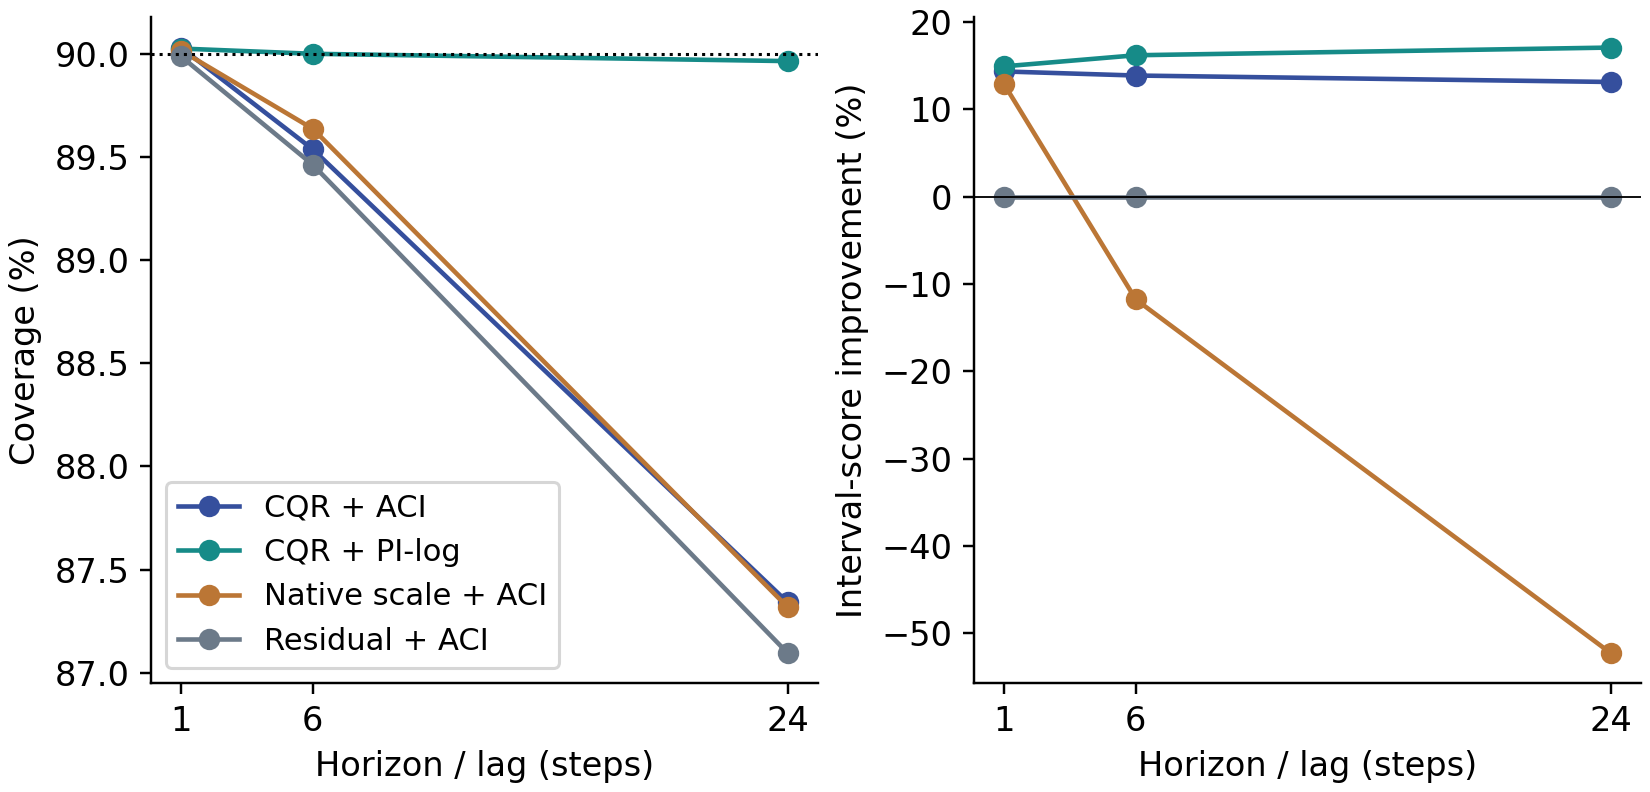
\includegraphics[width=\textwidth]{figures/horizon.png}
\caption{Joint changes in horizon and natural feedback delay on eight series and two
Chronos models. Coverage is an average; score gains use the horizon-specific residual--ACI
denominator. Solar steps are ten minutes, so $h=24$ is not day-ahead for those series.}
\label{fig:horizon}\end{figure}

The PI result is not a claim of uniformly improved reliability. At $h=24$, its local
150-origin coverage error is 4.86 percentage points, versus 4.52 for CQR--ACI. Improved
overall coverage can coexist with worse local variation. The controller also emits some
singletons after negative signed corrections: CQR--PI-log's average singleton rate is
0.567\% at $h=24$, versus 0.048\% for CQR--ACI. No infinite test intervals occur for
these two reported variants in this panel.

The fixed-forecast intervention separates lag from changing forecast difficulty
(Figure~\ref{fig:delay}). On the same $h=1$ predictions, increasing calibration lag from
1 to 24 steps changes residual--ACI coverage from 89.99\% to 88.62\% and CQR--ACI from
90.03\% to 89.52\%. CQR--PI-log remains at 89.99\% for lag 24, while its local coverage
error is 2.88 percentage points compared with 2.08 for CQR--ACI. Thus feedback restriction
alone can alter the relevant coverage comparison. The larger deficit in true $h=24$
forecasts additionally reflects changes in the forecast/score stream; lag alone does not
explain its entire magnitude.

\begin{figure}[htbp]\centering
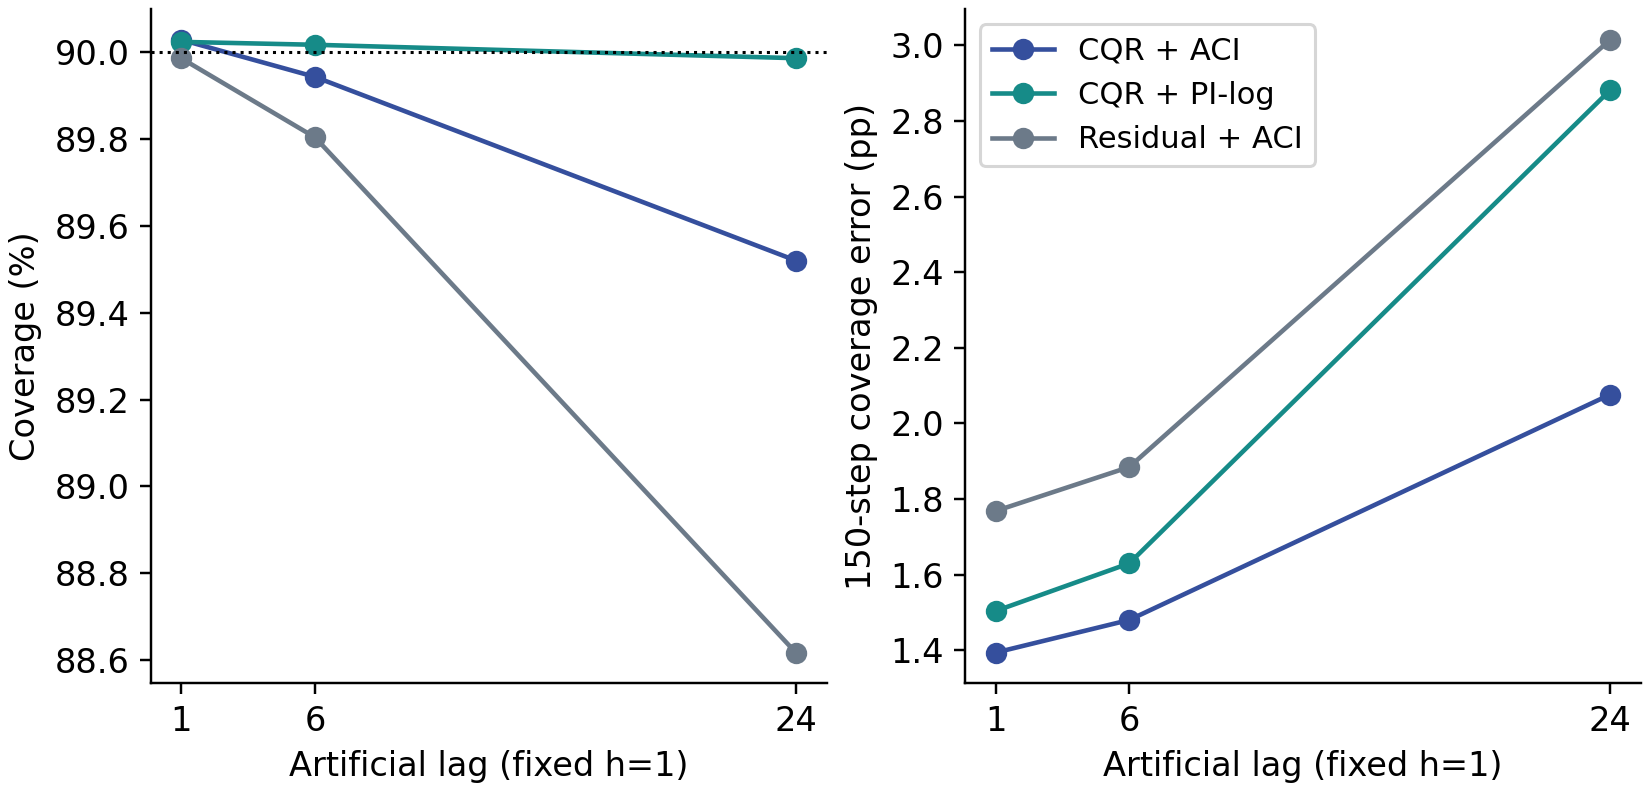
\includegraphics[width=\textwidth]{figures/delay_control.png}
\caption{Exploratory intervention holding one-step predictions and targets fixed while
withholding calibration outcomes. Overall coverage and local coverage error respond
differently. This isolates the calibrator's feedback channel, not the model's context.}
\label{fig:delay}\end{figure}

\subsection{Native information transfers across families}\label{sec:confirmresults}
Holding COP fixed, native CQR improves on residual scores by 12.27\%, 14.66\% and
22.16\% at $h=1,6,24$ on traffic and exchange rates. At $h=24$, family means are
11.10\% for exchange rates and 33.22\% for traffic; the exchange-rate mean exceeds
its median. Under original-grid issued ACI the gain is 8.50\%. These are matched
information contrasts, not improvements over all other controllers. Original
family contrasts are retained in \ref{app:confirmation}, with pair-level records in the artifact.
The scale of the benefit depends on the controller, motivating the state and rate
sensitivity below.

\subsection{Smaller rates explain most of the apparent CQR state advantage}\label{sec:rates}
The apparent CQR state gain is sensitive to the learning-rate range (Table~\ref{tab:rates}).
On development data, the $h=24$ CQR gain of issued over shared ACI falls from 6.54\%
to 0.73\% when both grids include $G_0/h$, and to 0.59\% under the wide grid.
Revisiting traffic and exchange rates yields the same pattern: 8.43\% falls to
1.27\% and 0.99\%, respectively. Thirteen of 16 paired differences remain positive,
but the large original effect is not robust to tuning adequacy. Wide-grid family
means are 0.52\% for exchange rates and 1.46\% for traffic. Broader tuning also does
not guarantee improved coverage: wide-grid means are 88.78\% for shared and 89.01\%
for issued CQR, below the 90\% target.
The wide grid still selects its minimum rate in 11/16 shared and 5/16 issued CQR
pairs on the revisited panel (7/16 for each state on development data); one revisited
issued pair selects its maximum. Thus this is a bounded sensitivity, not a claim
that the rate optima are bracketed. The grid was not expanded after these test results.

\begin{table}[htbp]\centering\scriptsize
\caption{Subsequent learning-rate sensitivity at $h=24$, CQR. Gain is issued versus
shared paired interval-score improvement (\%). S/I denote shared/issued states;
coverage is percent, and local error is in percentage points. Selection uses validation
only. The revisited panel is already inspected data, not a new confirmation test.}
\label{tab:rates}\begin{tabular}{llrrrrrr}
\toprule
Panel & Grid & Gain & Wins & Cov. S & Cov. I & Local S & Local I \\
\midrule
Development & original & 6.54 & 15/16 & 88.18 & 89.56 & 5.33 & 5.55 \\
Development & scaled & 0.73 & 13/16 & 89.54 & 89.35 & 5.62 & 5.60 \\
Development & wide & 0.59 & 13/16 & 89.45 & 89.32 & 5.66 & 5.61 \\
Traffic/FX & original & 8.43 & 16/16 & 87.87 & 89.43 & 5.79 & 6.12 \\
Traffic/FX & scaled & 1.27 & 13/16 & 89.00 & 89.03 & 6.14 & 6.25 \\
Traffic/FX & wide & 0.99 & 13/16 & 88.78 & 89.01 & 6.21 & 6.22 \\
\bottomrule
\end{tabular}

\end{table}

Native information remains useful after the grid expansion. On the revisited panel,
CQR improves over residual scores by 18.73\% under wide-grid shared ACI and by 9.80\%
under wide-grid issued ACI. The state effect also interacts with score construction:
wide-grid residual ACI retains an 11.34\% mean issued/shared improvement. Thus the
appropriate conclusion is a score--state--tuning interaction, not a universally large
advantage of issued-state updating. Equal candidate grids can obscure this interaction
when the admissible shared-state gain shrinks with delay.

The exact accounting in Equation~\eqref{eq:potential} makes the associated coverage
change measurable. For original-grid shared CQR on the revisited panel, the mean
revealed-test excess miscoverage is 2.150 percentage points: clipping contributes
2.117 and the endpoint term 0.033. With the scaled grid, clipping falls to 0.336
points while the endpoint contribution rises to 0.681. Smaller rates suppress the
observed clipping bias but leave a larger finite-time adaptation term. These are
exact decompositions of the emitted-error recursion, not proof that local linear
instability is the sole cause of interval-score differences. Pending test outcomes
are accounted for separately in \ref{app:rates}.

Controlled prescribed-response simulations further distinguish stability from tracking.
For $M_t(a)=\clip\{\alpha+g(a-a^*_t),0,1\}$, the shared state oscillates above its local
gain boundary, whereas issued updating can remain stable. At a smaller rate where
both structures are locally stable, issued updating can track a change more slowly.
These illustrations and the empirical rate--delay surfaces appear in \ref{app:rates};
they do not replace the stochastic, window-dependent behavior of the actual calibrators.

The configured multi-step PID has 88.03\% mean coverage and a 41.57\% higher
paired interval score than wide-grid issued CQR at $h=24$ on the revisited panel.
This complete-configuration comparison changes signed-error information, asymmetric
tail construction and controller dynamics simultaneously. It cannot attribute the
difference to the PID controller alone. The no-scorecaster ablation and full settings
are retained; neither comparison represents full AcMCP or an optimal scorecaster.

\subsection{Photovoltaic efficiency and reliability differ by output regime}
We first revisit the original one-step photovoltaic result on all eight plants and
four models, rather than inferring its explanation from a different long-horizon
panel. The original 35.25\% CQR--ACI gain is reproduced. Zero-output observations
account for 61.16\% of this test panel and contribute 19.64 percentage points of
the overall gain; positive-output observations contribute 15.61 points
(Table~\ref{tab:solarparts}). The positive-output conditional score itself improves
by 21.32\%. Its interval widths increase, but reduced lower/upper miss penalties
more than compensate. Thus the efficiency benefit is not confined to zeros.

\begin{table}[htbp]\centering\scriptsize
\caption{Original one-step PV decomposition, 32 model--series pairs. Share and coverage
are percent. Gain compares CQR with residual ACI within the listed group. Contribution
uses each pair's overall residual score as denominator, then averages; zero and positive
contributions sum to the overall gain. R denotes residual. Tuned rows reuse original
validation choices. Outcome groups are evaluation-only.}
\label{tab:solarparts}\begin{tabular}{llrrrrr}
\toprule
Settings & Group & Share & Gain & Contribution & Cov. R & Cov. CQR \\
\midrule
default & all & 100.00 & 35.25 & 35.25 & 89.88 & 89.96 \\
default & positive & 38.84 & 21.32 & 15.61 & 74.38 & 84.96 \\
default & zero & 61.16 & 73.37 & 19.64 & 99.72 & 93.14 \\
tuned & all & 100.00 & 20.51 & 20.51 & 89.34 & 89.72 \\
tuned & positive & 38.84 & 12.77 & 10.43 & 80.17 & 86.32 \\
tuned & zero & 61.16 & 54.89 & 10.08 & 95.16 & 91.88 \\
\bottomrule
\end{tabular}

\end{table}

Better positive-output score still does not imply target coverage: default CQR attains
\PVDefaultPositiveCoverage\% on positive outputs versus \PVDefaultOverallCoverage\% overall, although this is higher than the
residual method's 74.38\%. With matched original validation tuning, the overall gain
is 20.51\%, positive-output gain is \PVTunedPositiveGain\%, and positive-output coverage rises to
\PVTunedPositiveCoverage\% versus 80.17\% for residuals. Complete width and miss-penalty components are
reported in \ref{app:solarparts}. These results qualify the application claim without
discarding the observed efficiency benefit.

The separate long-horizon diagnostic concerns two other development photovoltaic
series and two backbones, so it is not a within-panel comparison with the one-step
decomposition.
On the two development photovoltaic series and two backbones, tuned CQR--COP at
$h=24$ attains 90.41\% overall coverage, yet only 79.93\% on positive-output targets
and 97.05\% on zero-output targets (Figure~\ref{fig:solarconditional}). Zero outputs
constitute approximately 61.04\% of these test segments. At $h=1$ and $h=6$,
positive-output coverage is 87.95\% and 82.42\%, respectively, despite overall coverage
near 90\%. These are four model--series pairs from two series, not four independent
solar datasets. Positive output is an outcome-defined diagnostic and need not
coincide with astronomical daytime. A marginal coverage theorem does not promise
coverage on this subset, so the finding is not a counterexample to that theorem.

\begin{figure}[!htbp]\centering
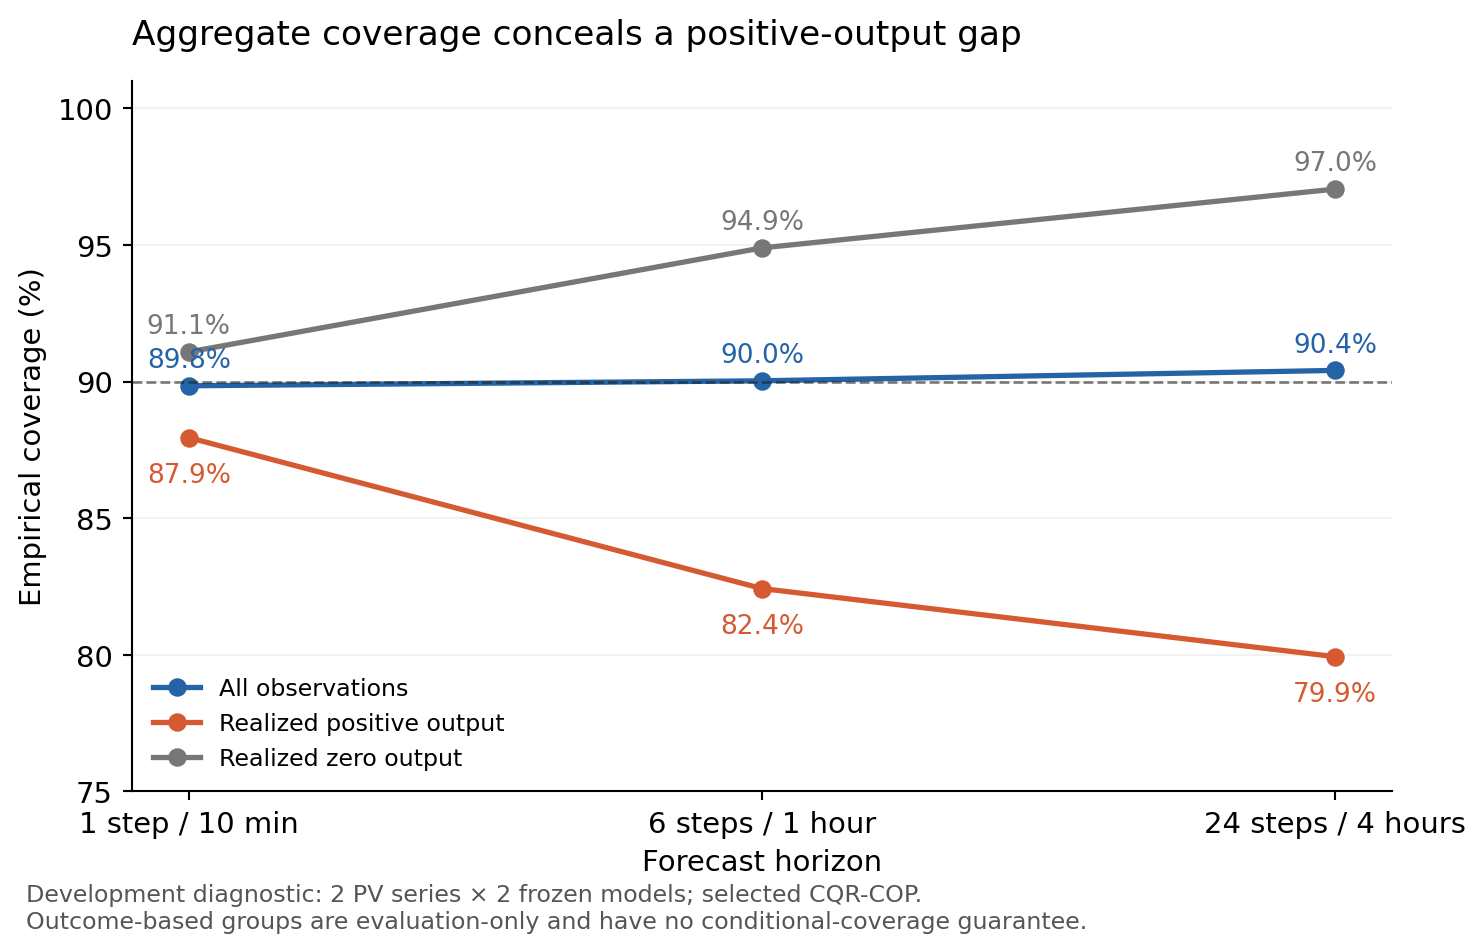
\includegraphics[width=\textwidth]{figures/solar_conditional_coverage.png}
\caption{Post-hoc photovoltaic reliability diagnostic for selected CQR--COP.
Coverages average over two series and two models. The zero/positive labels are used
only for evaluation; prediction and validation never use the future target label.
At this sampling rate, 24 steps represent four hours.}
\label{fig:solarconditional}\end{figure}

The observable-width grouping experiment tests whether a simple existing approach
can reduce the deficit. Separating both memory and state increases positive-output
coverage from 78.93\% to 83.49\% relative to matched shared-state CQR on these solar
pairs. Overall coverage changes from 88.46\% to 89.45\%, with a 2.47\% interval-score
gain. The positive-output gap remains substantial. Separating memory alone improves
solar interval score by 6.75\% but reduces overall coverage to 85.66\%, illustrating
why a proper-score change should be accompanied by coverage diagnostics.
Across all 16 development pairs, the both-grouped CQR gain is only 1.12\%.
On the confirmation families, the same grouping yields a 3.27\% gain at $h=24$,
but coverage remains 88.56\%, compared with 87.87\% for shared ACI. Grouping is thus
an informative control, not a demonstrated solution to conditional reliability.

Additional normalization, nominal-level and output-provenance sensitivities are
reported in \ref{app:sensitivity}; these qualify generalization beyond additive CQR.

\section{Discussion and limitations}
The practical result is a hierarchy of comparisons. First establish whether native
endpoints improve on point-only scores under a matched controller. Then assess
whether feedback adaptation adds enough over rolling calibration to justify its
score and reliability tradeoffs. Finally inspect relevant subgroups. In these
archives, native information survives the controls, a large CQR state gain does not
survive wider tuning, and positive-output undercoverage survives improved PV scores.
The clipping decomposition explains one concrete cost: smaller rates reduce the
accumulated projection correction but leave a larger finite-time endpoint term.
This links an implementation choice to observed coverage without assigning every
score change to local linear instability.

Scope limits remain material. The series are correlated; the panels include constructed
switches and only two models have multi-horizon archives. Public benchmark pretraining
exposure is unknown, and original main-panel checkpoint metadata are incomplete despite
exact spot-check agreement. The original confirmation uses a locally fixed protocol;
the subsequent sensitivities revisit inspected data. Frequent smallest-rate choices
mean the wide grid does not bracket every optimum. Thus the remaining 0.99\% mean
CQR state gain is not a precise, intrinsic contribution of state structure.

The information-matched comparisons and the complete PID configurations answer
different questions. Full AcMCP and O$^2$CP are not reproduced, and the fixed-default
variants in the unified table are not tuned optima. Neither this table nor the PID
comparison establishes state-of-the-art superiority. The midpoint/scale interventions
improve attribution but do not identify a universal causal law for heteroscedasticity.
The prescribed-response simulations are explanatory, and the artificial feedback lag
does not reproduce every consequence of a live sensor delay.

Finally, proper-score improvements are not conditional-coverage guarantees or reserve
procurement savings. The former needs stronger validity assumptions or a different
guarantee; the latter needs a specified decision policy and shortfall costs. Broader
independent deployments are needed to establish how far the observed tradeoffs transfer.

\section{Conclusion}
Native-band gains transfer beyond energy, but delayed-state advantages depend strongly
on tuning adequacy and score construction. Smaller shared-state rates explain most
of the initial long-horizon CQR difference; exact clipping accounting and controlled
tracking examples clarify the resulting tradeoff without asserting a new stochastic
validity theorem. Photovoltaic gains are not confined to zero outputs, yet improved
positive-output scores coexist with deficient coverage. Evaluation should separate
predictive information, state/rate choices and subgroup reliability, and disclose
common baselines and sensitivity status.

\section*{Data and code availability}
The accompanying software archive, Supplementary Software S1
(\texttt{Supplementary\_Software\_S1.zip}), contains a CPU reproduction entry point,
64 minimal forecast/target archives, fixed protocols and reference results.
\texttt{ARTIFACT\_MAP.md} identifies which manuscript tables and figures are rebuilt
and which historical results are supplied inputs. The rate, PID, photovoltaic and
simulation analyses replay in an isolated directory without model downloads or a GPU.
Neural prediction generation and the earlier full benchmark are outside that replay;
their provenance and result records are retained separately. Original data and model
terms remain applicable. The archive is prepared for reviewer access; a repository
URL will be added after author upload.

\section*{Funding}
This work is supported by the National Natural Science Foundation of China
(Grant No. 62372409).

\section*{Declaration of competing interest}
The authors declare no competing interests.

\section*{Declaration of generative AI and AI-assisted technologies}
OpenAI Codex assisted with literature retrieval, code auditing, experiment implementation,
analysis and preparation of this revised manuscript. The authors remain responsible
for reviewing the methods, results, citations and final text.

\clearpage
\appendix
\section{Dataset and archive details}\label{app:data}
UCI consumer indices are 5, 37, 70, 103, 136, 168, 201, 234, 267 and 300 in the public
LSTNet-format electricity matrix. Alabama plant indices are 3, 21, 39, 57, 75, 93, 111
and 130. Main observed traces use the initial 8,000 raw observations, except the two
minute-level ETT channels (12,000) and ERCOT channels (16,000). The ETT columns are
ETTh1/OT, ETTh2/OT, ETTm1/HUFL and ETTm2/OT.

The two cross-consumer splices concatenate 1,500-point segments starting at raw offset
1,000 from clients (10,40,70,100) and (25,90,140,210). Seasonal constructions use clients
20 and 80, concatenating 1,200-point windows starting at offsets 4392, 8784, 13128 and
17544. They deliberately omit the intervening chronology. Synthetic series have length
6,000, seeds 1 and 7, AR coefficient 0.7, a sinusoid of period 200 and four piecewise
mean/innovation-scale regimes $(0,1),(0,2.2),(5,0.8),(-3,1.6)$.

The multi-horizon panel uses electricity clients 20 and 80, solar plants 10 and 30,
ETTh1/OT, the first cross-consumer splice, seasonal client 20 and synthetic seed 1.
Origins stop 24 steps before the raw-series end for every horizon, ensuring the same
origins within that panel. Public data sources are the LSTNet data repository\footnote{\url{https://github.com/laiguokun/multivariate-time-series-data}},
ETDataset\footnote{\url{https://github.com/zhouhaoyi/ETDataset}}, ERCOT historical
load\footnote{\url{https://www.ercot.com/gridinfo/load/load_hist}} and GEFCom2014.

\clearpage
\section{Detailed delayed-feedback results}
\begin{table}[h!]\centering\small
\caption{Multi-horizon comparison. Gains use the residual--ACI score at the same horizon.
Local error is in percentage points. Tuning never uses test labels.}
\label{tab:horizon}\begin{tabular}{lrrr}
\toprule
Horizon / method & Gain (\%) & Cov. (\%) & Local (pp) \\
\midrule
1 / residual/aci & 0.00 & 89.99 & 1.77 \\
1 / native-scale/aci & 12.91 & 90.01 & 1.31 \\
1 / cqr/aci & 14.35 & 90.03 & 1.39 \\
1 / cqr/pi-log & 14.94 & 90.02 & 1.50 \\
1 / cqr/saocp & 12.48 & 90.69 & 2.10 \\
1 / cqr/faci & 15.42 & 89.61 & 1.68 \\
1 / cqr/aci/tuned & 14.87 & 90.09 & 1.97 \\
6 / residual/aci & 0.00 & 89.46 & 2.44 \\
6 / native-scale/aci & -11.77 & 89.64 & 1.96 \\
6 / cqr/aci & 13.89 & 89.54 & 2.06 \\
6 / cqr/pi-log & 16.21 & 90.00 & 2.53 \\
6 / cqr/saocp & 5.26 & 84.09 & 6.13 \\
6 / cqr/faci & 15.50 & 86.74 & 3.81 \\
6 / cqr/aci/tuned & 15.47 & 89.74 & 3.13 \\
24 / residual/aci & 0.00 & 87.10 & 4.90 \\
24 / native-scale/aci & -52.27 & 87.32 & 4.50 \\
24 / cqr/aci & 13.15 & 87.34 & 4.52 \\
24 / cqr/pi-log & 17.09 & 89.96 & 4.86 \\
24 / cqr/saocp & 6.56 & 79.98 & 10.16 \\
24 / cqr/faci & 15.57 & 82.72 & 7.94 \\
24 / cqr/aci/tuned & 11.62 & 88.09 & 5.46 \\
\bottomrule
\end{tabular}
\end{table}

\clearpage
\section{Per-series primary comparison}
\begin{table}[h!]\centering\small
\caption{Default CQR--ACI compared with default residual--ACI, averaged over four backbones.}
\begin{tabular}{lrr}
\toprule
Series & Gain (\%) & Coverage (\%) \\
\midrule
ETTh1\_OT & 3.12 & 89.98 \\
ETTh2\_OT & 8.27 & 89.99 \\
ETTm1\_HUFL & 8.74 & 89.99 \\
ETTm2\_OT & 3.70 & 89.97 \\
electricity\_c103 & 5.21 & 89.97 \\
electricity\_c136 & 4.87 & 89.99 \\
electricity\_c168 & 5.90 & 89.93 \\
electricity\_c201 & 5.33 & 89.96 \\
electricity\_c234 & 6.61 & 90.00 \\
electricity\_c267 & 4.74 & 90.01 \\
electricity\_c300 & 17.21 & 89.91 \\
electricity\_c37 & 8.05 & 89.97 \\
electricity\_c5 & 8.43 & 89.95 \\
electricity\_c70 & 5.72 & 89.89 \\
ercot\_COAST & 0.77 & 90.01 \\
ercot\_ERCOT & -1.53 & 90.00 \\
ercot\_NORTH & 1.86 & 89.97 \\
seasonal\_elec\_c20 & 6.25 & 90.09 \\
seasonal\_elec\_c80 & 10.90 & 90.00 \\
solar\_p111 & 34.92 & 89.90 \\
solar\_p130 & 34.37 & 89.92 \\
solar\_p21 & 36.12 & 89.97 \\
solar\_p3 & 35.42 & 89.97 \\
solar\_p39 & 35.01 & 90.07 \\
solar\_p57 & 35.63 & 89.94 \\
solar\_p75 & 36.33 & 89.98 \\
solar\_p93 & 34.21 & 89.97 \\
spliced\_electricity\_4seg & 11.36 & 90.10 \\
spliced\_electricity\_4seg\_b & 13.27 & 90.02 \\
synthetic\_T6000 & 0.31 & 89.99 \\
synthetic\_T6000\_s7 & -0.42 & 90.02 \\
\bottomrule
\end{tabular}
\end{table}

\clearpage
\section{Confirmation controller diagnostics}\label{app:confirmation}
\begin{table}[htbp]\centering\scriptsize
\caption{Confirmation contrasts at $h=24$. Each row contains four series and two models.
Gain and median are paired interval-score improvements (\%); A is the first method in
the comparison and B the second. Coverage is in percent, target 90\%. Correlated pairs
are retained without interpreting the win count as independent replications.}
\label{tab:confirmation}\begin{tabular}{llrrrrr}
\toprule
Comparison & Family & Gain & Median & Wins & Cov. A & Cov. B \\
\midrule
Native / residual, COP & FX & 11.10 & 2.73 & 7/8 & 89.76 & 89.72 \\
Native / residual, COP & Traffic & 33.22 & 31.79 & 8/8 & 90.45 & 91.40 \\
Native / residual, issued ACI & FX & 3.79 & 1.06 & 8/8 & 89.03 & 89.10 \\
Native / residual, issued ACI & Traffic & 13.20 & 11.92 & 8/8 & 89.83 & 90.20 \\
Issued / shared, CQR & FX & 8.62 & 5.01 & 8/8 & 89.03 & 86.12 \\
Issued / shared, CQR & Traffic & 8.24 & 7.98 & 8/8 & 89.83 & 89.63 \\
\bottomrule
\end{tabular}

\end{table}

\begin{table}[h!]\centering\scriptsize
\caption{Unified comparison on the revisited panel at $h=24$. IS ratio averages
per-pair interval scores divided by that pair's residual rolling-quantile score;
lower is better. Family coverage is percent (target 90\%). Local is the family-balanced
150-origin absolute coverage error in percentage points; Singleton is percent.
Original rows retain locked-grid results, wide ACI and multi-step PID are subsequent
sensitivities. PI-log and SF-OGD retain fixed defaults, not tuned optima.}
\begin{tabular}{llrrrrr}
\toprule
Score & Controller & IS ratio & FX cov. & Traffic cov. & Local & Singleton \\
\midrule
Residual & Rolling & 1.000 & 87.48 & 89.58 & 6.77 & 0.000 \\
Residual & Shared, original & 1.063 & 87.75 & 88.51 & 5.66 & 0.000 \\
Residual & Issued, original & 0.929 & 89.10 & 90.20 & 6.58 & 0.000 \\
Residual & Shared, wide & 1.066 & 87.57 & 88.07 & 6.14 & 0.000 \\
Residual & Issued, wide & 0.939 & 88.53 & 89.72 & 6.57 & 0.000 \\
Residual & PI-log & 2.341 & 89.92 & 90.03 & 6.36 & 2.873 \\
Residual & SF-OGD & 5.146 & 90.18 & 90.03 & 6.63 & 4.356 \\
Residual & COP & 1.177 & 89.72 & 91.40 & 6.39 & 0.249 \\
Residual & Grouped ACI & 0.984 & 86.76 & 89.23 & 5.74 & 0.000 \\
Residual & Fixed-scale OGD & 1.096 & 86.11 & 90.50 & 7.14 & 0.344 \\
Residual & Implicit-delay & 1.057 & 86.05 & 90.03 & 6.98 & 0.000 \\
CQR & Rolling & 0.852 & 87.78 & 89.41 & 6.37 & 0.038 \\
CQR & Shared, original & 0.937 & 86.12 & 89.63 & 5.79 & 0.167 \\
CQR & Issued, original & 0.853 & 89.03 & 89.83 & 6.12 & 0.025 \\
CQR & Shared, wide & 0.860 & 88.02 & 89.53 & 6.21 & 0.031 \\
CQR & Issued, wide & 0.851 & 88.14 & 89.88 & 6.22 & 0.044 \\
CQR & PI-log & 2.048 & 90.04 & 89.98 & 6.06 & 3.011 \\
CQR & SF-OGD & 4.528 & 90.17 & 90.09 & 6.47 & 4.377 \\
CQR & COP & 0.879 & 89.76 & 90.45 & 5.57 & 0.028 \\
CQR & Grouped ACI & 0.904 & 87.45 & 89.67 & 5.62 & 0.018 \\
CQR & Fixed-scale OGD & 0.884 & 88.25 & 90.92 & 6.13 & 0.126 \\
CQR & Implicit-delay & 0.884 & 88.33 & 90.92 & 6.07 & 0.069 \\
Signed error & Multi-step PI & 1.163 & 86.89 & 89.22 & 6.68 & 0.024 \\
Signed error & Multi-step PID & 1.176 & 86.85 & 89.21 & 6.92 & 0.065 \\
\bottomrule
\end{tabular}

\end{table}

\clearpage
\section{Algorithm and integrity checks}\label{app:integrity}
The primary evidence concerns the archived forecasts, not a reranking of freshly
downloaded checkpoints. Offline spot checks reproduce the point and five quantile outputs
exactly at 21 selected origins per model across three main-panel series, for 84 checked
model--origin cases. For the two Chronos models, matching the original default batch
grouping of 256 contexts resolves differences observed with a seven-context batch.
TimesFM's checked outputs match the local 2.0 checkpoint through its Hugging Face adapter;
Moirai matches after its original quantile-rearrangement step. Current checkpoint hashes
and environment versions are recorded. These checks support archive provenance but
do not constitute a rerun of every forecast, and original checkpoint commits were not
stored with every archive. Possible pretraining exposure to
public benchmark data also precludes an assertion that all test series were unseen during
pretraining.


The executable checks test future-target perturbations at lags 1, 6 and 24, identical
evaluation masks, unit rescaling, exact stored-level selection, empirical quantile
agreement, interval-score arithmetic, finite behavior under zero-width forecasts and
the reference SAOCP expert recursion. Data validation independently reconstructs target
values from local raw-series loaders. Cache records include archive, protocol and code
hashes; aggregations reject stale code/protocol outputs.

Source implementations and licenses are retained for SAOCP/FACI and PID. The SAOCP
numerical check covers its nonnegative-score expert recursion, without validating a
theorem for signed or delayed extensions. Appendix~\ref{app:rules} specifies controller
conventions; the artifact retains complete grids, failures and tail misses. Recorded
runtimes include possible compilation overhead and do not measure neural inference speed.

Additional checks cover clipping identities, COP source-recursion equivalence,
target/issue-time conversion, grouped feedback assignment and implicit proximal
optimality against an independent optimizer and subgradient conditions. Protocols
and exploratory amendments remain separately identifiable.

The asymmetric multi-step PID comparison matches the unmodified author implementation
over 24 horizons and four configured scorecasters, including future-target perturbations.
Check records and tolerances accompany the artifact; full AcMCP remains incomplete.

\clearpage
\section{Matched implicit-update ablation}\label{app:implicit}
The implicit ablation exactly solves the proximal objective already considered by
\citet{hu2026cop}. With $p=1-\alpha$, pinball loss $\ell_p(u)=u(p-\ind\{u<0\})$,
and a fixed prefix-scaled step $\eta=\gamma(\max_{i<600}s_i-\min_{i<600}s_i)$
(range floored at $10^{-12}$), it uses
\begin{equation}\label{eq:prox}
 b_t=b_{t-1}+\eta(e_{t-h}-\alpha),\qquad
 q_t=\arg\min_q\left\{\frac{(q-b_t)^2}{2}
       +h\eta\,\widehat{\mathbb E}_t[\ell_p(S-q)]\right\}.
\end{equation}
The same 300-score convention supplies the empirical distribution. The matched OGD
ablation sets $q_t=b_t$. Both select from $\{0.005,0.02,0.05,0.1\}$ and these values
divided by $h$. The point of this control is to distinguish an implicit correction's
incremental value from the fixed scale and learning rate. The development screen also
retains half-step and explicit corrections; it did not validate a new algorithm.

The delay-scaled implicit correction in Equation~\eqref{eq:prox} has a plausible
stationary rationale. If the true and proxy CDFs have local densities $g>0$ and
$\widehat g\geq0$, its deterministic linearized delayed gain is
$c=\eta g/(1+h\eta\widehat g)$. With a correct slope it is below $1/h$ and hence
inside the classical shared-state stability boundary in Equation~\eqref{eq:stability}.
For fixed slopes, however, this is simply a smaller effective gain. It predicts no
automatic advantage over suitably tuned basic gradient updating, and the argument
does not cover changing empirical distributions or atoms.

The development screen evaluates 3,200 configuration instances, retaining every
setting. At $h=24$, implicit-delay CQR improves interval score by 2.54\% over issued
ACI and 2.08\% over delay-tuned COP, but only 0.23\% over matched fixed-scale OGD.
It fails the locally recorded continuation criterion of at least 3\% against both
strong baselines, even before further validation. On the subsequent confirmation
panel, its matched-OGD gain is $-0.08\%$: $-0.30\%$ for exchange rates and $0.14\%$
for traffic, with seven of 16 positive differences. We therefore retain this result
as a negative ablation, not a new main method. A more sophisticated update formula
is insufficient evidence of additional predictive information or better adaptation.


\clearpage
\section{Rate, delay and clipping diagnostics}\label{app:rates}
Figure~\ref{fig:ratesurface} uses the common ten-rate subset of the wide grid to
display the rate--delay sensitivity. It shows every listed rate's test behavior,
not a test-based selector. The original selected shared-state CQR score at each
horizon is a common per-pair denominator for both structures. The additional
delay-scaled rates also participate in selection and remain in the full result files.

\begin{figure}[htbp]\centering
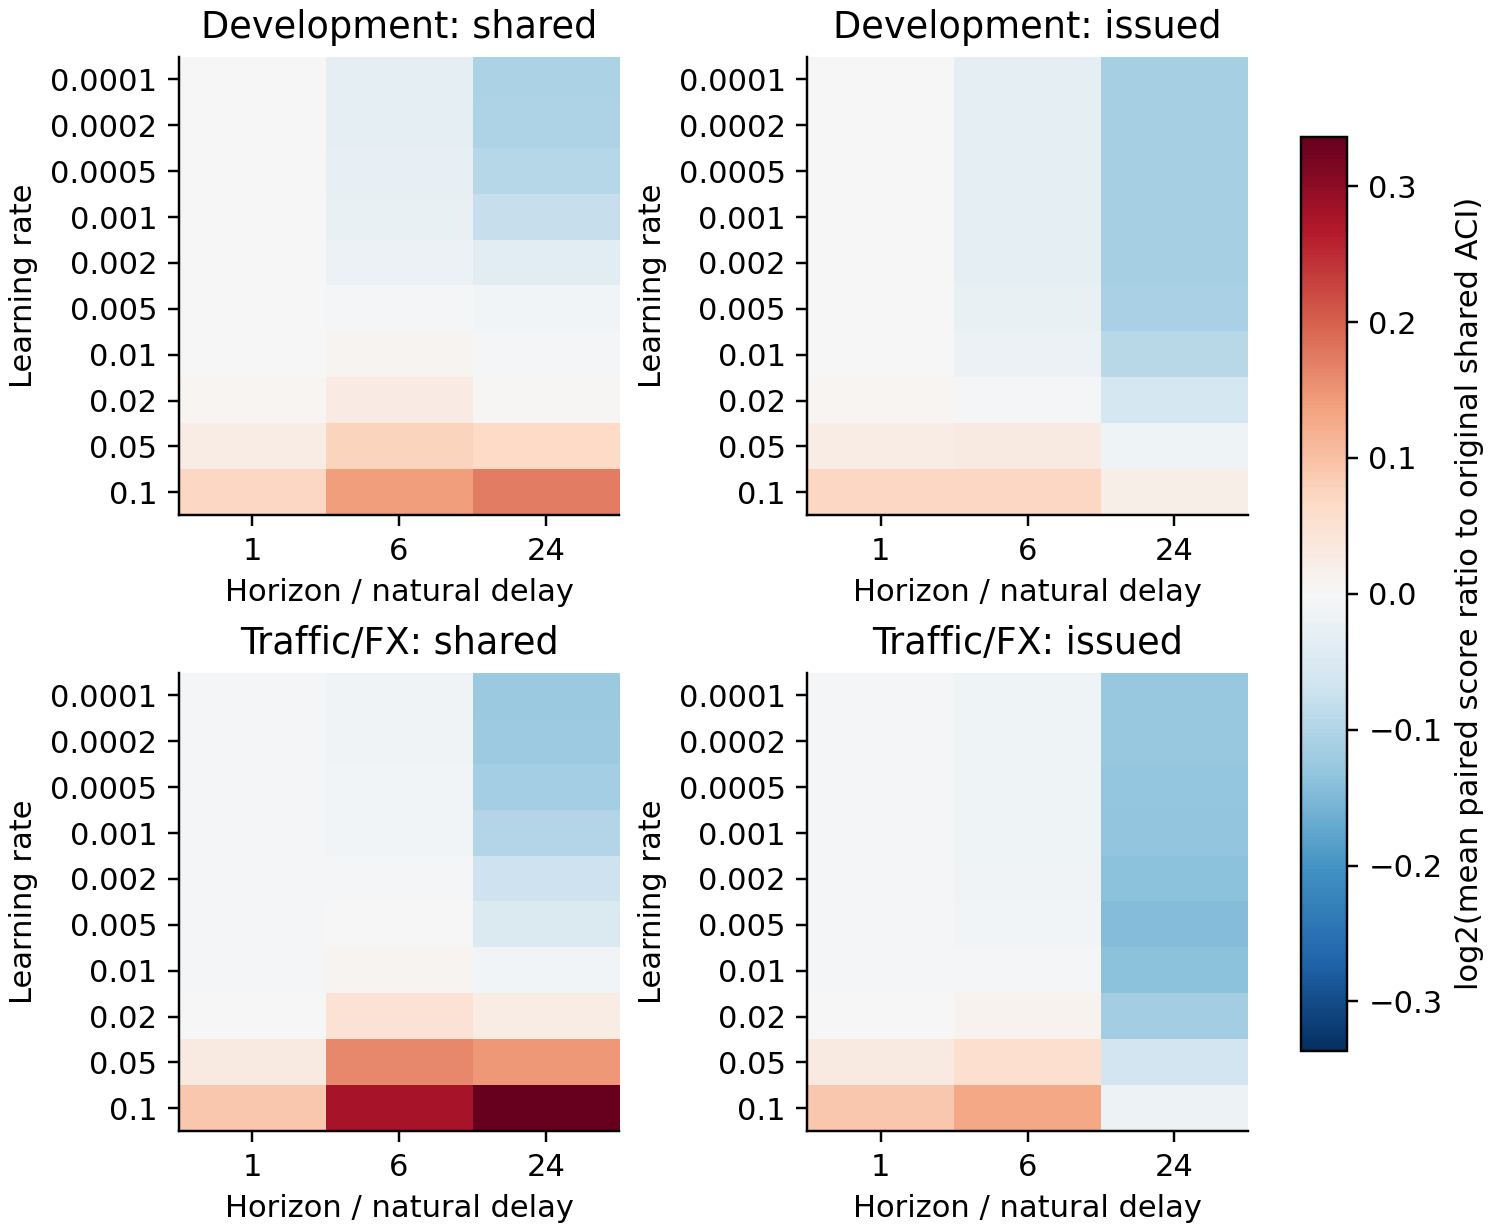
\includegraphics[width=\textwidth]{figures/rate_delay_surface.png}
\caption{CQR rate--delay surfaces. Color is the base-two logarithm of the mean
paired interval-score ratio to original-grid shared CQR; zero means equal score.
Positive values are worse. Development and revisited panels have 16 pairs each.
Validation selects configurations; the plotted test surface is descriptive.}
\label{fig:ratesurface}\end{figure}

\begin{table}[htbp]\centering\scriptsize
\caption{Exact revealed-test miscoverage decomposition, CQR, $h=24$, in percentage
points. Clip plus Endpoint equals Excess up to rounding. Each interval was issued
in the test segment and revealed by the last archive origin. The last 24 issued
test intervals are pending; their separately recorded contribution bounds the
difference from full issued-test coverage by $24/N_{\rm test}$.}
\begin{tabular}{lllrrr}
\toprule
Panel & Grid & State & Clip & Endpoint & Excess \\
\midrule
Development & original & shared & 1.801 & 0.004 & 1.804 \\
Development & original & issued & 0.023 & 0.393 & 0.415 \\
Development & scaled & shared & 0.043 & 0.398 & 0.441 \\
Development & scaled & issued & 0.023 & 0.611 & 0.633 \\
Development & wide & shared & 0.043 & 0.487 & 0.530 \\
Development & wide & issued & 0.023 & 0.642 & 0.664 \\
Traffic/FX & original & shared & 2.117 & 0.033 & 2.150 \\
Traffic/FX & original & issued & 0.135 & 0.461 & 0.596 \\
Traffic/FX & scaled & shared & 0.336 & 0.681 & 1.017 \\
Traffic/FX & scaled & issued & 0.135 & 0.863 & 0.998 \\
Traffic/FX & wide & shared & 0.336 & 0.909 & 1.245 \\
Traffic/FX & wide & issued & 0.182 & 0.834 & 1.016 \\
\bottomrule
\end{tabular}

\end{table}

For the controlled simulations, the response is prescribed as
$M_t(a)=\clip\{0.1+g(a-a_t^*),0,1\}$, with $g\in\{1,4\}$ and $h\in\{1,6,24\}$.
Runs contain 12,000 steps. Stationary runs use effective gains at 0.5 and 1.2 times
the shared linear boundary. Tracking runs use $a_t^*=0.1,0.2,0.06$ in three
4,000-step segments and the original three rates plus their delay-scaled versions.
Deterministic response feedback and Bernoulli feedback are kept distinct, with
20 fixed seeds for the latter, yielding 1,764 controller runs. In the deterministic
$h=24,g=4,\gamma=0.005$ tracking example, mean absolute state error over the first
500 steps after both changes is 0.0198 for shared and 0.0978 for issued updating.
This is a specified-response illustration, not a forecast score or a causal diagnosis
of all empirical losses.

\begin{figure}[htbp]\centering
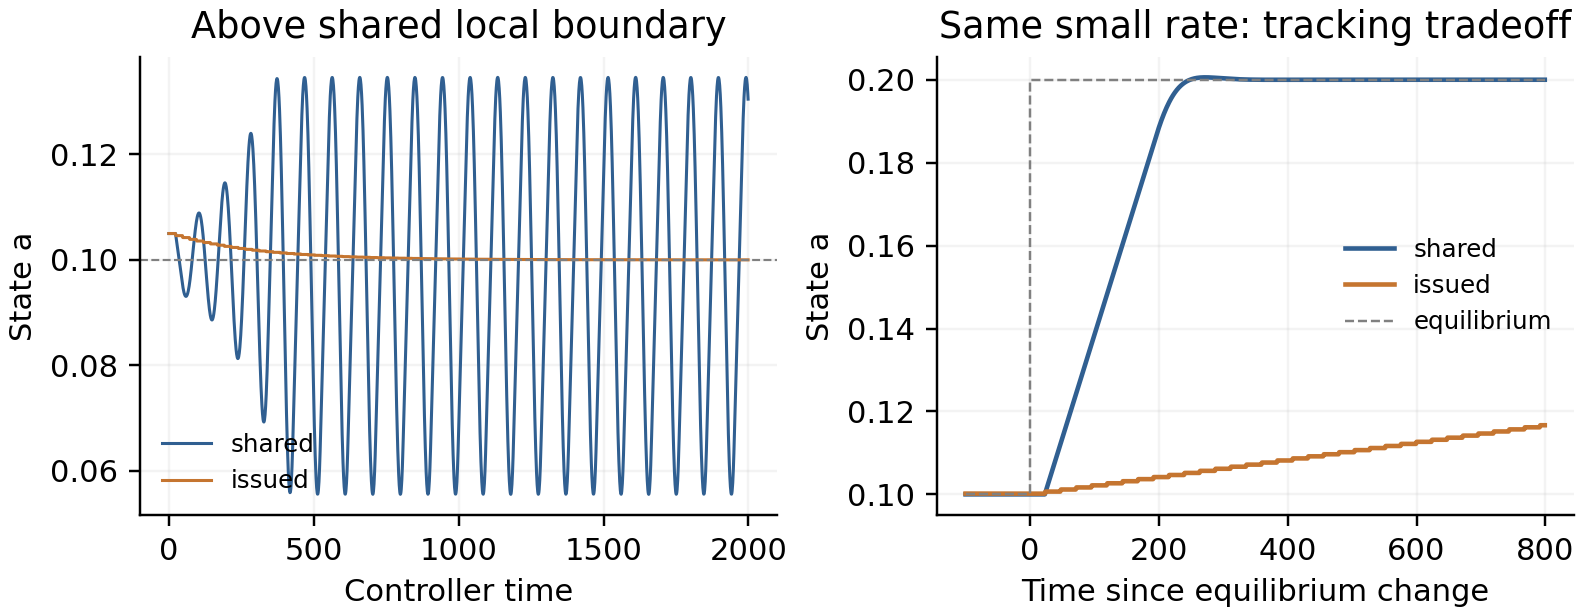
\includegraphics[width=\textwidth]{figures/controlled_dynamics.png}
\caption{Deterministic response illustrations at $h=24,g=4$. Left: effective gain
1.2 times the shared local boundary. Right: $\gamma=0.005$, below the boundary for
both states, following an equilibrium change. State clipping and response saturation
are explicit; the trajectories illustrate stability and tracking, not coverage guarantees.}
\label{fig:dynamics}\end{figure}

\clearpage
\section{Photovoltaic score components}\label{app:solarparts}
\begin{table}[htbp]\centering\small
\caption{One-step PV interval-score components, averaged over the original 32 pairs.
IS equals Width plus Lower plus Upper, where the last two are the $2/\alpha$-weighted
miss-distance penalties. These means use the shared PV data units; the headline
relative gains are instead calculated per pair before averaging. All outcome-defined
groups are evaluation-only.}
\begin{tabular}{lllrrrr}
\toprule
Settings & Score & Group & IS & Width & Lower & Upper \\
\midrule
default & cqr & all & 2.629 & 1.766 & 0.555 & 0.308 \\
default & cqr & positive & 5.978 & 3.831 & 1.386 & 0.761 \\
default & cqr & zero & 0.498 & 0.454 & 0.025 & 0.020 \\
default & residual & all & 4.046 & 2.284 & 1.218 & 0.544 \\
default & residual & positive & 7.607 & 3.086 & 3.126 & 1.395 \\
default & residual & zero & 1.781 & 1.773 & 0.006 & 0.002 \\
tuned & cqr & all & 2.575 & 1.816 & 0.476 & 0.282 \\
tuned & cqr & positive & 5.888 & 4.017 & 1.183 & 0.688 \\
tuned & cqr & zero & 0.467 & 0.417 & 0.027 & 0.023 \\
tuned & residual & all & 3.240 & 1.987 & 0.820 & 0.432 \\
tuned & residual & positive & 6.775 & 3.626 & 2.066 & 1.082 \\
tuned & residual & zero & 0.991 & 0.945 & 0.027 & 0.019 \\
\bottomrule
\end{tabular}

\end{table}
Each pair's all-observation score and coverage is reconstructed by weighting its
zero- and positive-output components by their own sample fractions. This check is
performed before any averaging across plants and models. There are no negative
targets in this evaluated PV panel. The original default and validation-tuned
overall scores are reproduced from the archived predictions before decomposition.

\clearpage
\section{Additional sensitivities}\label{app:sensitivity}
\subsection{Scale mismatch can amplify interval widths}
Normalization is helpful when the predicted scale tracks error size. It can also amplify
historical mistakes. For positive scales, a native-normalized residual interval has width
\begin{equation}\label{eq:ratio}
 2\tilde b_t\,Q_{1-a_t}\!\left(\{|y_i-m_i|/\tilde b_i:i\in\mathcal H_t\}\right).
\end{equation}
If more than the upper-tail fraction of the calibration history has error magnitude $c$
and scale $\varepsilon$, its empirical threshold can approach $c/\varepsilon$. A later
scale $B$ then produces width $2Bc/\varepsilon$. A relative floor keeps the expression
finite, but does not eliminate a large historical-to-current scale ratio. Additive CQR
does not have this particular multiplicative amplification mechanism, although it can
still perform poorly when the base endpoints or update rule are unsuitable.

This argument does not establish that every normalization loss is caused by exact zero
bands. Both scale transitions and very small but nonzero widths matter. We therefore
retain all failures, record floor activation and score extremes, and avoid a test-dependent
score cap. Nor does the argument establish that a proposed regularizer must improve
prediction: the validation and test experiments must decide that question.

\subsection{Normalization failures and unsuccessful selection}
At $h=24$, native-scale ACI has a mean gain of $-52.27\%$, despite a 12.91\% gain on
the same panel at $h=1$. Large losses occur on the Chronos-Bolt solar series and on
constructed scale switches, as well as smaller losses elsewhere. For example, its
interval-score increase on Chronos-Bolt/solar-p10 is 286.35\% relative to residual--ACI.
These cases are consistent with historical-to-current scale mismatch in
Equation~\eqref{eq:ratio}; exact zero bands are not required. The artifacts include
width-floor activation rates and normalized-score extremes for every trace.

Regularized normalized CQR does not reliably fix the problem. Across all three horizons,
its mean gains range from $-12.50\%$ at $\lambda=0$ to $-9.65\%$ at $\lambda=1$ for the
reported endpoint choices, compared with 13.80\% for additive CQR--ACI. The validation
selector increases the main-panel gain from 13.57\% to 13.72\%, but its multi-horizon
mean is 13.36\%, below fixed CQR--ACI. We retain this failed hypothesis instead of
expanding the selector grid on the test results. Prefix-based selection remains causal,
but a causal procedure need not transfer well across later regimes.

\subsection{Nominal levels, rearrangement and native-output provenance}
The primary CQR--ACI benefit persists at 80\% and 95\% calibrated targets
(Table~\ref{tab:sensitivity}). Omitting quantile rearrangement changes the primary mean
gain from 13.57\% to 13.56\%. The main conclusion is therefore not driven by sorting,
although sorting matters more for some individual normalized-score configurations.

\begin{table}[htbp]\centering\small
\caption{CQR--ACI sensitivity, using default residual--ACI at the same nominal level as
the denominator. Dense archives are a repeated-output sensitivity, not new independent data.}
\label{tab:sensitivity}\begin{tabular}{lrrr}
\toprule
Panel / miscoverage & Pairs & Gain (\%) & Cov. (\%) \\
\midrule
main-a0.2 & 124 & 9.85 & 80.01 \\
main-a0.1 & 124 & 13.57 & 89.98 \\
main-a0.05 & 124 & 14.00 & 94.90 \\
dense-a0.1 & 93 & 13.80 & 89.98 \\
gefcom-a0.1 & 39 & 19.63 & 89.99 \\
\bottomrule
\end{tabular}
\end{table}

The genuine stored 0.1--0.9 native bands achieve average main-panel coverage of 81.89\%
(Chronos-2), 87.04\% (Chronos-Bolt), 81.96\% (Moirai) and 77.57\% (TimesFM), against
their 80\% nominal mass. These values include both overcoverage and undercoverage.
They cannot substantiate a claim that all models' native 90\% intervals under-cover.

The dense archive requires additional care. TimesFM still stores only the five original
levels, so it supplies no genuine 0.05--0.95 comparison. Chronos-Bolt's stored 0.05 and
0.95 outputs equal its 0.1 and 0.9 outputs on approximately 99.86\% of rows after
rearrangement; requesting more levels did not create independent tail information.
Chronos-2's stored 0.05--0.95 band attains 91.69\% coverage at a nominal 90\%.
We therefore do not use the dense files to claim exact full-distribution CRPS or a
universal native 90\% calibration result.

\setlength{\bibsep}{4pt}

\clearpage
\section{Controller implementation details}\label{app:rules}
\subsection{One-step and delayed rule variants}
We compare seven rules using the same score streams and observation schedule.
\begin{enumerate}
\item \emph{Split}: a fixed empirical $(1-\alpha)$ quantile of the initial 600 scores.
\item \emph{Rolling}: an empirical $(1-\alpha)$ quantile of the latest $W=450$ revealed scores.
\item \emph{Clipped ACI}: replace $\alpha$ in the rolling quantile by $a_t$, updated as
\begin{equation}\label{eq:aciappendix}
 a_t=\clip_{[0.001,0.999]}\{a_{t-1}+\gamma(\alpha-e_{t-d})\},\qquad \gamma=0.02,
\end{equation}
where $e_i=\ind\{y_i\notin C_i\}$ and the update is applied only after an issued interval's
outcome becomes available. The equation suppresses idle steps before that event.
\item \emph{SF-OGD adaptation}: with $M=\max_{i<600}|s_i|$, update the threshold by
$q\leftarrow q-Mg/\sqrt{\sum g^2}$, where $g=\alpha-e$. We initialize at the prefix
quantile and allow signed thresholds. This coverage-gradient implementation is described
explicitly rather than claimed identical to every tie/projection convention in the
published wrapper \citep{bhatnagar2023saocp}.
\item \emph{PI-log adaptation}: a proportional threshold update and logarithmic tangent
integrator inspired by \citet{angelopoulos2023pid}. With $k$ revealed post-initialization
errors and $E_k=\sum_{j=1}^k(e_j-\alpha)$,
\begin{equation}\label{eq:pi}
 z_k=z_{k-1}+\gamma M(e_k-\alpha),\qquad
 q_k=z_k+M\tan\!\left(E_k\frac{\log(k+2)}{k+1}\right).
\end{equation}
The tangent saturates to signed infinity outside $(-\pi/2,\pi/2)$. The initial $z$ is the
prefix quantile. We use a fixed prefix scale, omit scorecasting and retain our causal
delay convention; this is not full reference PID.
\item \emph{SAOCP adaptation}: the strongly adaptive coin-betting expert update from
the author implementation \citep{bhatnagar2023saocp}, with default lifetime multiplier 8
and prefix scale $\sqrt{3}M$. The accelerated residual-score implementation agrees
numerically with an independent driver of the original expert class. For signed CQR we
remove its nonnegative projection; with delayed feedback, experts process scores in
reveal order. These are declared extensions, without transferring the original theorem
to the modified setting.
\item \emph{FACI-R}: the author's FACI aggregation update with eight learning rates
$0.001\,2^j$, $j=0,\ldots,7$, fixed-share mixing and a rolling 450-score empirical survival
function. Unlike a full-history wrapper, this variant deliberately shares the rolling
history design. Its weighted level is inverted using the empirical inverted-CDF quantile.
\end{enumerate}
The first five rules use linear empirical quantile interpolation where applicable.
Consequently, ``split'' denotes the fixed-threshold comparator here; we do not assert
the exact finite-sample rank correction or exchangeability guarantee of textbook split
conformal prediction for these dependent streams.

For ACI, we separately select $(\gamma,W)$ from
$\{0.005,0.02,0.05\}\times\{200,450,900\}$ using only the validation prefix.
The score selector retains the declared default rule settings. We report fixed defaults
and tuned controls separately, rather than describing one untuned baseline as optimal.


\subsection{Optimistic and groupwise controls}
The exact COP reference recursion is checked numerically against the author's
implementation. Our delayed adaptation is distinct: at issue $t$, with $j=t-h$,
it uses the preceding 300 revealed scores, excluding $s_j$, to form the empirical
CDF $\widehat F_t$ and step scale $R_t=\max s-\min s$. After feedback starts, it updates
\begin{equation}\label{eq:cop}
 b_t=b_{t-1}+\eta_t(e_j-\alpha),\qquad
 q_t=b_t-\tfrac12\eta_t\{\widehat F_t(b_t)-(1-\alpha)\},\quad \eta_t=\ell R_t.
\end{equation}
It starts from the 0.9 quantile of the 600-score prefix; before the first issued
interval's feedback arrives, the threshold stays at that initial value.
Validation selects $\ell$ from $\{0.05,0.1,0.5,1\}$ and those values divided by $h$.
The divided-rate extension was added after inspecting the development panel and is
explicitly exploratory there. It was fixed before the confirmation evaluation.
Singleton repairs use actual emitted-interval feedback; the original COP guarantees
are not asserted for this delayed, repaired adaptation.

Grouped ACI is an established groupwise-calibration control \citep{vovk2005algorithmic}.
The grouping feature is native band width, with a threshold fixed at its median in
the first 600 forecasts; ties enter the low-width group. The development factorial
separates score memory, feedback state, both, or neither. Group memory retains 450
scores per group and falls back to global history with fewer than 20 observations.
Each revealed error updates the state assigned at its issue time. Confirmation uses
the version with both memory and state separated, with the same ACI rate grid.

The matched implicit-update control and its negative result are specified in
\ref{app:implicit}.


\subsection{Configured multi-step PID}
We also compare the asymmetric multi-step PID implementation supplied with AcMCP
\citep{wang2026acmcp,angelopoulos2023pid}. Its two tails target $\alpha/2$, retain the
author's zero internal initialization and warmup recursion, and use error-range-scaled
steps and the unbounded tangent integral correction. We set rolling history to 600,
$C_{\rm sat}=0.5$, and initialize $K_I$ to the maximum absolute error revealed in the
first 600 target-clock rows across horizons 1--24, rather than using the whole trace.
Validation selects the rate from $\{0.005,0.01,0.05,0.1\}$ and those rates divided by
$h$, jointly with no scorecaster, a rolling mean, the author's documented naive
scorecaster, or a declared least-squares AR(1). The latter clips the fitted coefficient
to $[-0.995,0.995]$, recalculates the intercept from sample means, and iterates $h$ steps.
It is a configured scorecaster, not the author's default or an AcMCP substitute.

An accelerated implementation reproduces the unmodified author recursion on one
1,000-origin electricity archive for all 24 horizons and four scorecasters, and passes
future-target perturbation checks. The benchmark evaluates all 32 development/revisited
pairs and all three horizons, totaling 2,560 configurations. Crossed endpoints are
collapsed to their midpoint for evaluation, while the internal tail-score feedback is
preserved for source fidelity. Infinite or invalid intervals receive infinite score
rather than being omitted. A separately selected no-scorecaster control is retained.


\bibliographystyle{elsarticle-num-names}
\bibliography{references}
\end{document}
